%\VignetteDepends{MAMA,methods, metaArray, xtable, metaMA, gtools, gplots, multtest, RankProd, MergeMaid, GeneMeta} 
% \VignetteIndexEntry{An R Package for Meta-Analysis of Microarray}
% \VignetteKeywords{Microarray}
% \VignettePackage{MAMA}

\documentclass[a4paper]{report}

\title{MAMA: an R package for Meta-Analysis of MicroArray}
\author{Ivana Ihnatova}

\usepackage{Sweave}
\begin{document}

\maketitle
\tableofcontents
\newpage
\chapter{Introduction}
%It is well-known that analysis of microarray is statistically difficult and results differ even in repeated experiments.  \par

%By combining data sets from different origins together, the test gets increased power, which leads to more identified genes \cite{Hong}.


%There are three main objectives in analysis of microarray: class comparison (finding of differentially expressed genes), class prediction (prognostic prediction) and class discovery (clustering or unsupervised analyses). 
This paper provides a user guide to R-package MAMA. The package implements eight different methods that have been proposed in meta-analysis of microarray and are designed to identify differentially expressed genes.\par


In here, we will demonstrate the features of the package with an example of meta-analysis in cancer microarray data, the comparison of expression profiles in MSI (microsatelite instable) and MSS (microsatelite stable) colon cancer. We gathered three microarray data from public databases. The data are stored in {\ttfamily ColonData}. It is an object of new S4 class - {\ttfamily MetaArray}, in which separate slots for gene expression data matrices (expression profiles), clinical sample characteristics and datanames were defined. \par
We start with package and sample data loading. 
\begin{Schunk}
\begin{Sinput}
> rm(list=ls(all=TRUE))
> options(width=60)
> library(MAMA)
> data(ColonData)
> ColonData
\end{Sinput}
\begin{Soutput}
Dataset Denmark  containing 500 probes and  77 samples. 
Sumarization of samples: 
MSIstatus 
--------- 
MSI MSS 
 39  38 
age 
--- 
   Min. 1st Qu.  Median    Mean 3rd Qu.    Max. 
  36.00   45.00   54.00   54.92   62.00   80.00 

Dataset Australia  containing 500 probes and  36 samples. 
Sumarization of samples: 
MSIstatus 
--------- 
MSI MSS 
  5  31 
age 
--- 
   Min. 1st Qu.  Median    Mean 3rd Qu.    Max. 
  50.00   57.75   66.00   66.36   73.75   85.00 

Dataset Japan  containing 500 probes and  41 samples. 
Sumarization of samples: 
location 
-------- 
  distal proximal  unknown 
      28       11        2 
MSIstatus 
--------- 
MSI MSS 
 16  25 
age 
--- 
   Min. 1st Qu.  Median    Mean 3rd Qu.    Max. 
  40.00   47.00   53.00   53.61   60.00   65.00 
\end{Soutput}
\end{Schunk}
The original data sets have been preprocessed and subsampled in order to reduce the computational complexity of the meta-analysis. All data sets have been normalized and are in $log_2$-scale. The corresponding sample sizes for the three datasets can be seen in outprint above. The same set of 500 gene has been selected in each dataset.\par 
A different method is described in each of the parts below and the descriptions are independed from each other, so you can directly move to the method of your interest. Meta-analysis usually consist of three steps: Data preparation, Detection of differentially expressed genes and Extraction and visualization of results. There is also a wrapper function for each method that outperforms all necessary step as one-line command.\par
We select the significant genes at significance level of 0.05 in all methods. 
 
\chapter{Methods that combine p-values}
%\addcontentsline{toc}{part}{Methods that combine p-values}
\section*{Introduction}
%\addcontentsline{toc}{section}{Introduction}
In this part we will focus on methods that combine p-values \cite{Marot}, \cite{Rhodes}. These methods are inspired by Fisher's S-statistic published in 1925 \cite{Fisher25}. \par
Two measurements of significance of change in gene expression are the most common. These are: value of test-statistic and p-value. In here the p-values from study-specific analysis are combined into one p-value in sense of sum of logs. Methods differ in test statistic used to calculate the study-specific p-values. 
\section*{Usage}
%\addcontentsline{toc}{section}{Usage}
\subsection*{Data preparation}
One needs a list of gene expression data matrices {\ttfamily esets} and a list of vectors with class labels {\ttfamily classes}. The former is {\ttfamily GEDM} slot of MetaArray object, the latter can be obtained by function {\ttfamily selectClass}. 
\begin{Schunk}
\begin{Sinput}
> esets <- GEDM(ColonData)
> classes <- selectClass(ColonData, "MSIstatus", "factor")
\end{Sinput}
\end{Schunk}
\subsection*{Detecting differentially expressed genes}
Functions \verb!pvalcombination! and \verb!pvalcombination.paired! provide meta-analysis based on combination of p-values. The first one is designed for unpaired data and the second for paired design of microarray experiments. Because, our data sets are unpaired, we will use \verb!pvalcombination!. The function requires: a list of gene expression data matrices ({\ttfamily esets}), a list of vectors of class labels ({\ttfamily classes}), type of test statistics ({\ttfamily moderated}) and threshold for significance ({\ttfamily BHth}). It returns list of indices of selected genes. Three possible values for argument {\ttfamily moderated} are available: {\ttfamily "t"} for common t-test, {\ttfamily "limma"} for moderated t-test used in {\ttfamily limma} package \cite{limma} and {\ttfamily "SMVar"} for moderated t-test defined in SMVar package \cite{SMVar}. 
\begin{Schunk}
\begin{Sinput}
> pvalt<-pvalcombination(esets, classes, moderated = "t" , BHth = 0.05)
\end{Sinput}
\begin{Soutput}
    DE    IDD   Loss    IDR    IRR 
215.00  43.00  20.00  20.00  10.42 
\end{Soutput}
\end{Schunk}
Several characteristics, which have been defined in meta-analysis of microarray (especially for methods which combine p-values or effect sizes), are outprinted by the function. {\ttfamily DE} denotes number of significant genes in meta-analysis. {\ttfamily IDD} represents Integration Driven Discoveries, it means genes which are significant in meta-analysis but not in any of the individual studies. Other way round, if a gene is significant only in individual data sets but not in meta-analysis, it is called Integration Driven Revision and {\ttfamily Loss} is a number of such genes. {\ttfamily IDR} and {\ttfamily IRR} are percentages of Integration Driven Discoveries and Integration Driven Revisions in identified differentially expressed genes ({\ttfamily DE}).  
%pvallimma<-pvalcombination(esets, classes, moderated = "limma" , BHth = 0.01)
%pvalSMVar<-pvalcombination(esets, classes, moderated = "SMVar" , BHth = 0.01)
\subsection*{Results}
\begin{Schunk}
\begin{Sinput}
> summary(pvalt)
\end{Sinput}
\begin{Soutput}
              Length Class  Mode   
study1        162    -none- numeric
study2         14    -none- numeric
study3         99    -none- numeric
AllIndStudies 192    -none- numeric
Meta          215    -none- numeric
TestStatistic 500    -none- numeric
\end{Soutput}
\end{Schunk}
This object is a list with six slots. \emph{Study1} to \emph{Study3} are numeric vectors with indices of differentially expressed genes in data sets 1 to 3. \emph{AllIndStudies} is a vector of indices of differentially expressed genes in at least one data set. Differentially expressed genes found by meta-analysis have their indices stored in \emph{Meta}. And finally, a slot called \emph{TestStatistic} is a vector with test statistics in meta-analysis.  
\subsection*{Wrapper function}
Function {\ttfamily metaMA} is a wrapper funcion for this method. It does not require the data preparation step and returns the same ouput as {\ttfamily pvalcombination}. By
\begin{Schunk}
\begin{Sinput}
> pval<- metaMA(ColonData, "MSIstatus", which ="pval")
\end{Sinput}
\begin{Soutput}
    DE    IDD   Loss    IDR    IRR 
212.00  43.00  22.00  20.28  11.52 
\end{Soutput}
\end{Schunk}
we combine study specific p-values({\ttfamily pval}) in {\ttfamily ColonData} dataset using column {\ttfamily "MSIstatus"} from clinical data as class labels. The only difference between {\ttfamily pval} and {\ttfamily pvalt} is the \emph{gene.names} slot in the wrapper function.
%\section*{Discussion}
%\addcontentsline{toc}{section}{Discussion}

\chapter{Methods that combine effect sizes}
%\addcontentsline{toc}{part}{Methods that combine effect size}
\section*{Introduction}
%In the situation where $k$ microarray data sets are available and we want to estimate the mean difference in expression, for each gene, between two classes (e.g MSI and MSS colon cancer).\par
Methods that combine effect size use hierarchical model:
\[ y_i=\theta_i+\epsilon_i, \epsilon_i \sim N(0,\sigma_i^2)\]
\[ \theta_i=\mu+\delta_i, \delta_i \sim N(0,\tau_i^2),\]
where $\mu$ is true difference in mean expression between two classes, $y_i$ denotes the measure effect for study $i$, with $i=1,..,k$, $\tau^2$ represents the between study variability, $\sigma_i^2$ denotes the within study variability. The analysis is different depending on whether a fixed-effect model (FEM) or a random-effect model (REM) is deemed appropriate. Under a FEM, $\tau=0$ is assumed, otherwise a REM need to be fit. The estimates of the overall effect $\mu$ are different depending on which model is used. \par
Two papers dealing with effect size combination as method for meta analysis of microarray have been published \cite{Marot} and \cite{Choi2003}. They differ in effect size definition and implementation.\par 
Method presented in \cite{Marot} offers three variants of effect sizes (classical and moderated T-test) and uses explicitly random-effect model. It is implemented as two functions {\ttfamily EScombination} for unpaired data and {\ttfamily EScombination.paired} for paired data.  
\par On the other hand, in \cite{Choi2003} the effect size is defined as Hedge's and Olkin's $g$ and both random-effect and fixed-effect are available. Package \emph{GeneMeta} \cite{GeneMeta} implements this method. 
\section*{Algorithm}
\begin{enumerate}
\item Data recoding.
\item Effect size calculation in each data set.
\item Decision between random-effect model (REM) and fixed-effect model (FEM).
\item Model application.
\item Identification of differentialy expressed genes.
\end{enumerate}
%\addcontentsline{toc}{section}{Introduction}
\section*{Usage}
Because there are two different ways of implementation of this method, we will discuss them separately.
%\addcontentsline{toc}{section}{Usage}
\subsection*{Implementation from metaMA package}
\paragraph{Data preparation}
This method requires two lists, one containing the data matrices and the other one the corresponding vectors of group labels.
\begin{Schunk}
\begin{Sinput}
> esets <- GEDM(ColonData)
> classes <- selectClass(ColonData, "MSIstatus", "factor")
\end{Sinput}
\end{Schunk}
\paragraph{Detecting differentially expressed genes}
As we have unpaired data, we are going to use function {\ttfamily EScombination}. This function has four arguments: a list of gene expression data matrices ({\ttfamily esets}), a list of class labels vectors ({\ttfamily classes}), effect size definition ({\ttfamily moderated})  and a threshold for false discovery rate (FDR) ({\ttfamily BHth}). Three possible values for {\ttfamily moderated} are available: {\ttfamily "t"} for common t-test, {\ttfamily "limma"} for moderated t-test used in limma package \cite{limma} and {\ttfamily "SMVar"} for moderated t-test defined in SMVar package \cite{SMVar}. 
\begin{Schunk}
\begin{Sinput}
> ESt<-EScombination(esets, classes, moderated = "t" , BHth = 0.01)
\end{Sinput}
\begin{Soutput}
    DE    IDD   Loss    IDR    IRR 
109.00  28.00  51.00  25.69  38.64 
\end{Soutput}
\end{Schunk}
Function {\ttfamily EScombination} prints several measures defined in meta-analysis of microarray. {\ttfamily DE} denotes number of significant genes in meta-analysis. {\ttfamily IDD} represents Integration Driven Discoveries, it means genes which are significant in meta-analysis but not in any of the individual studies. Other way round, if a gene is significant only in individual data sets but not in meta-analysis, it is called Integration Driven Revision and {\ttfamily Loss} is a number of such genes. {\ttfamily IDR} and {\ttfamily IRR} are percentages of Integration Driven Discoveries and Integration Driven Revisions in identified differentially expressed genes ({\ttfamily DE}). 
\begin{Schunk}
\begin{Sinput}
> summary(ESt)
\end{Sinput}
\begin{Soutput}
              Length Class  Mode   
study1        113    -none- numeric
study2          8    -none- numeric
study3         59    -none- numeric
AllIndStudies 132    -none- numeric
Meta          109    -none- numeric
TestStatistic 500    -none- numeric
\end{Soutput}
\end{Schunk}
This object is a list with six slots. \emph{Study1} to \emph{Study3} are indices of differentially expressed genes in data sets 1 to 3. \emph{AllIndStudies} is a vector of indices of differentially expressed genes in at least one data set. Differentially expressed genes found by meta-analysis have their indices stored in \emph{Meta}. And finally, a slot called \emph{TestStatistic} is a vector with test statistics ("combined effect size") in meta-analysis. 
\paragraph{Wrapper function}
The same results can be obtained via
\begin{Schunk}
\begin{Sinput}
> es <- metaMA(ColonData, "MSIstatus", which = "ES")
\end{Sinput}
\begin{Soutput}
    DE    IDD   Loss    IDR    IRR 
166.00  27.00  52.00  16.27  27.23 
\end{Soutput}
\end{Schunk}

\subsection*{Implemenetation from GeneMeta package}
\paragraph{Data preparation}
Before calculating effect sizes we have to create numeric vectors with class labels in form of $1$'s and $0$'s. $1$ is supposed to be for diseased samples and $0$ for normal samples. In data sets used as example in this document $1$ refers to MSI samples and $0$ to MSS.  
\begin{Schunk}
\begin{Sinput}
> ph1<-clinical(ColonData)[[1]][,1]
> levels(ph1) <- c(1, 0)
> clinical(ColonData)[[1]][,1]
\end{Sinput}
\begin{Soutput}
 [1] MSI MSI MSI MSI MSI MSI MSI MSI MSI MSI MSI MSI MSI MSI
[15] MSI MSI MSI MSI MSI MSI MSI MSI MSI MSI MSI MSI MSI MSI
[29] MSI MSI MSI MSI MSI MSI MSI MSI MSI MSI MSI MSS MSS MSS
[43] MSS MSS MSS MSS MSS MSS MSS MSS MSS MSS MSS MSS MSS MSS
[57] MSS MSS MSS MSS MSS MSS MSS MSS MSS MSS MSS MSS MSS MSS
[71] MSS MSS MSS MSS MSS MSS MSS
Levels: MSI MSS
\end{Soutput}
\begin{Sinput}
> ph1
\end{Sinput}
\begin{Soutput}
 [1] 1 1 1 1 1 1 1 1 1 1 1 1 1 1 1 1 1 1 1 1 1 1 1 1 1 1 1 1
[29] 1 1 1 1 1 1 1 1 1 1 1 0 0 0 0 0 0 0 0 0 0 0 0 0 0 0 0 0
[57] 0 0 0 0 0 0 0 0 0 0 0 0 0 0 0 0 0 0 0 0 0
Levels: 1 0
\end{Soutput}
\end{Schunk}
\begin{Schunk}
\begin{Sinput}
> ph2<-clinical(ColonData)[[2]][,1]
> levels(ph2) <- c(1, 0)
> ph3<-clinical(ColonData)[[3]][,2]
> levels(ph3) <- c(1, 0)
> 
\end{Sinput}
\end{Schunk}
{\ttfamily ph1}, {\ttfamily ph2} and {\ttfamily ph3} are numeric vectors containing class labels for data sets {\ttfamily denmark}, {\ttfamily australia} and {\ttfamily japan}.  These vectors are needed as arguments for functions which provide effect size and its variability estimates. 

\paragraph{Detecting differentially expressed genes}
Functions {\ttfamily getdF}, {\ttfamily dstar} and {\ttfamily sigmad} estimate effect size and its variability for a individual data set, therefore we have to use them three-times. For {\ttfamily denmark} data set  
\begin{Schunk}
\begin{Sinput}
> d.den <- getdF(GEDM(ColonData)[[1]], ph1)
> d.adj.den <- dstar(d.den, length(ph1))
> var.d.adj.den <- sigmad(d.adj.den, sum(ph1 == 0), sum(ph1 == 1))
> head(d.adj.den)
\end{Sinput}
\begin{Soutput}
[1]  0.4835090 -0.1882238 -0.2740332 -0.4466879 -0.9850491
[6] -1.1694108
\end{Soutput}
\begin{Sinput}
> head(var.d.adj.den)
\end{Sinput}
\begin{Soutput}
[1] 0.05347487 0.05218687 0.05244444 0.05325247 0.05825761
[6] 0.06083683
\end{Soutput}
\end{Schunk}
and for other two data sets 
\begin{Schunk}
\begin{Sinput}
> d.aus <- getdF(GEDM(ColonData)[[2]], ph2)
> d.adj.aus <- dstar(d.aus, length(ph2))
> var.d.adj.aus <- sigmad(d.adj.aus, sum(ph2 == 0), sum(ph2 == 1))
> d.jap <- getdF(GEDM(ColonData)[[3]], ph3)
> d.adj.jap <- dstar(d.jap, length(ph3))
> var.d.adj.jap <- sigmad(d.adj.jap, sum(ph3 == 0), sum(ph3 == 1))
\end{Sinput}
\end{Schunk}
Function {\ttfamily getdF} has two arguments: the data set (a ExpressionSet object or a matrix) and class labels (a factor or numeric vector with $1$ and $0$) and computes estimates of standardized mean difference, found in Hedge and Olkin's \cite{Hedges}. Function {\ttfamily dstar} corrects the estimates for sample size bias, therefore its second argument is sample size of the data set. Function {\ttfamily sigmad} calculates the estimate of variance of unbiased effect size. For calculation, the user has to provide effect size estimates and sample size of each class. \par
Now, we are going to use Chochran's $Q$ statistic \cite{Cochran} to test between-study variability, so we can decide whether we should be considering random-effect (REM) or fixed-effect model(FEM) for the data. \par
Function {\ttfamily f.Q} provides a straightforward calculation of Cochran's $Q$ statistic. If the null hypothesis that the between-study variance is equal to zero (data are well modeled by a fixed effects design) then the estimated Q values will have approximately a chi-squared distribution with degrees of freedom equal to the number of studies minus one. We are going to look at mean and histogram of $Q$ statistics. Later we will compare quantiles of $Q$ to quantiles of chi-square distribution.  

\begin{center}
\begin{Schunk}
\begin{Sinput}
> mymns <- cbind(d.adj.den, d.adj.aus,d.adj.jap)
> myvars <- cbind(var.d.adj.den, var.d.adj.aus,var.d.adj.jap)
> my.Q <- f.Q(mymns, myvars)
> mean(my.Q)
\end{Sinput}
\begin{Soutput}
[1] 2.576469
\end{Soutput}
\begin{Sinput}
> hist(my.Q, breaks = 50, col = "red")
\end{Sinput}
\end{Schunk}
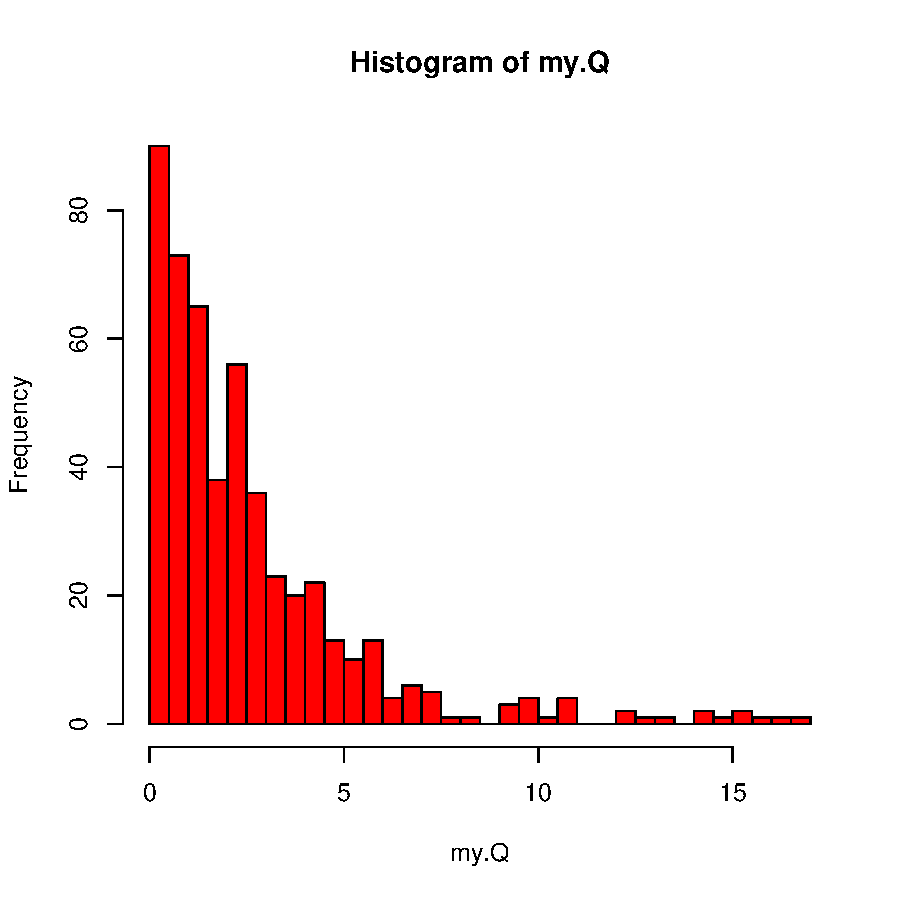
\includegraphics{MAMA_full-014}
\end{center}
\begin{center}
\begin{Schunk}
\begin{Sinput}
> num.studies <- 3
> plotQvsChi(my.Q, num.studies)
\end{Sinput}
\end{Schunk}
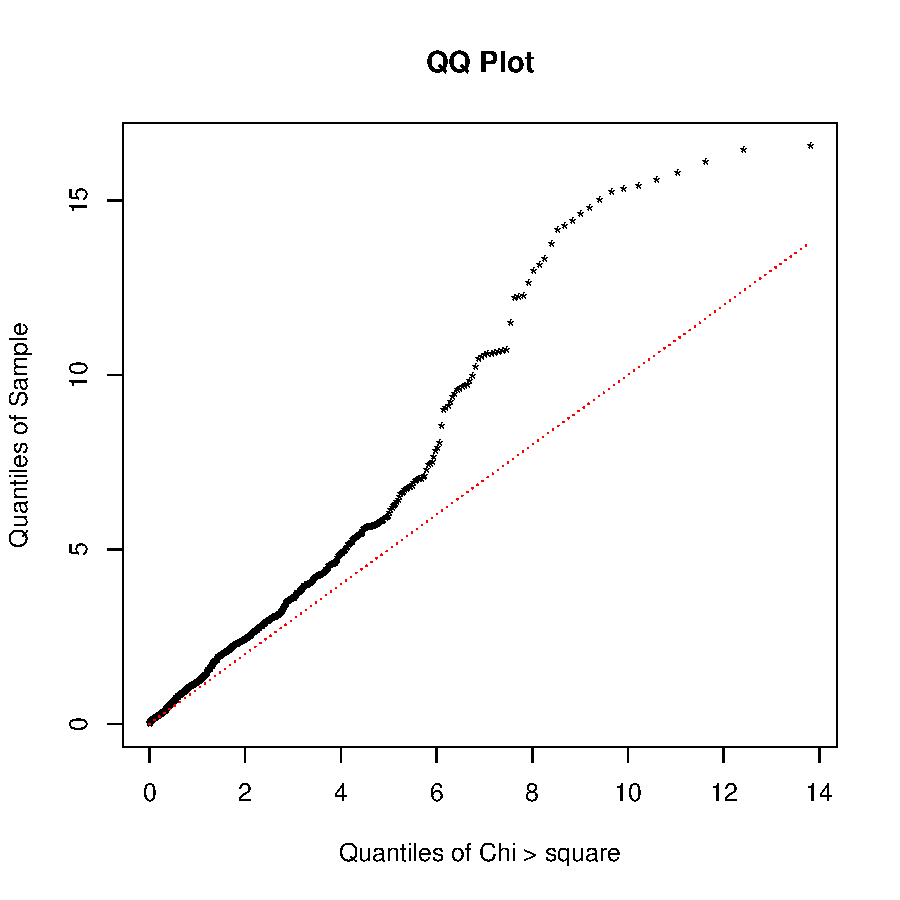
\includegraphics{MAMA_full-015}
\end{center}
According to Q-Q plot the hypothesis seems to be valid and fixed-effect model (FEM) should be used. However, we are going to use random-effect model (REM) too, so we can see if there is any difference in estimates of combined effect size.\par  
The computation is simpler for FEM than for REM. Functions {\ttfamily mu.tau2} and {\ttfamily var.tau2} estimate combined effect size ({\ttfamily mu.tau2}) and variance ({\ttfamily var.tau2}). Each effect size is a weighted average of the effects for the individual data sets divided by its standard error. The weights are the reciprocal of the estimated variances.  

\begin{center}
\begin{Schunk}
\begin{Sinput}
> #FEM
> muFEM = mu.tau2(mymns, myvars)
> sdFEM = var.tau2(myvars)
> ZFEM = muFEM/sqrt(sdFEM)
> qqnorm(ZFEM, pch = "*")
> qqline(ZFEM, col = "red")
\end{Sinput}
\end{Schunk}
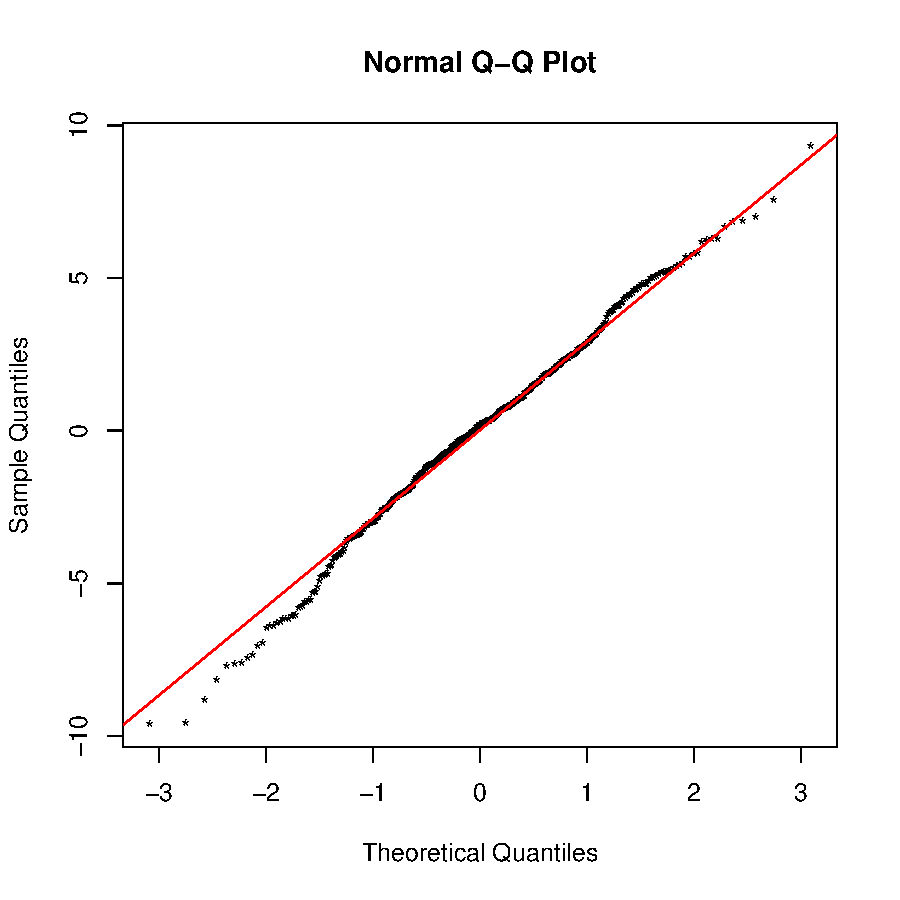
\includegraphics{MAMA_full-016}
\end{center}

Plotting the quantiles of the effects we can see that the presumption of approximate Normality seems to be appropriate.\par
In REM we have to account between-study variability ($\tau^2$). Function {\ttfamily tau2.DL} provides DerSimonian's and Laird's \cite{DerSimonian} estimates of $\tau^2$ from Cochran's $Q$. It has two addional arguments: number of studies ({\ttfamily num.studies}) and weights ({\ttfamily my.weights=1/myvars}). We add between-study variability to estimated variance ({\ttfamily myvars}) and calculate the combined effect size like in FEM.
\begin{Schunk}
\begin{Sinput}
> #REM
> num.studies <- 3
> my.tau2.DL <- tau2.DL(my.Q, num.studies, my.weights=1/myvars)
> myvarsDL <- myvars + my.tau2.DL
> muREM <- mu.tau2(mymns, myvarsDL)
> varREM <- var.tau2(myvarsDL)
> ZREM <- muREM/sqrt(varREM)
\end{Sinput}
\end{Schunk}
{\ttfamily muFEM} or {\ttfamily muREM} are numeric vectors with estimated combined (overall) effect size for a gene in FEM or REM. The estimated standard error of overall effect size for each gene is stored in numeric vectors: {\ttfamily varFEM} or {\ttfamily varREM}. We will test significance of overall effect size by Z-score ({\ttfamily ZFEM} or {\ttfamily ZREM}) defined as mean divided by standard error.\par
We can easily compare FEM estimates and REM estimates
\begin{center}
\begin{Schunk}
\begin{Sinput}
> plot(muFEM, muREM, pch = "*")
> abline(0, 1, col = "red")
\end{Sinput}
\end{Schunk}
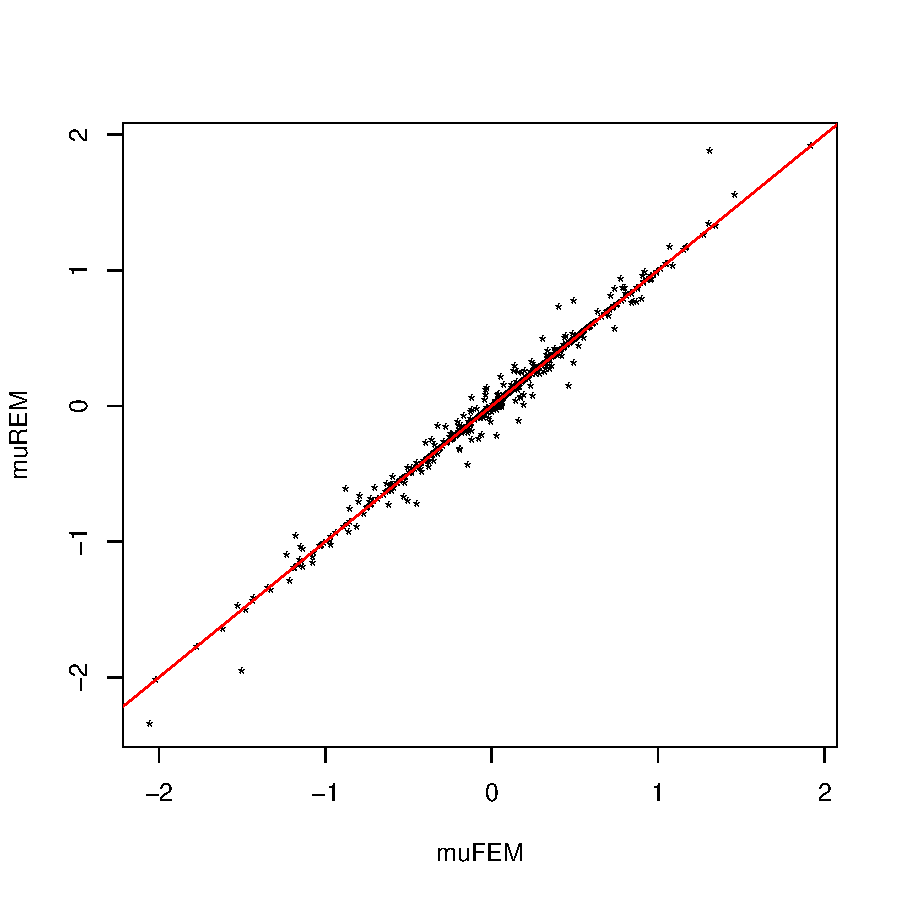
\includegraphics{MAMA_full-018}
\end{center} 
We do not see much difference here. Actually, for most of the genes the $\tau^2$ is estimated as zero. 
\begin{center}
\begin{Schunk}
\begin{Sinput}
> hist.tau<-hist(my.tau2.DL, col = "red", breaks = 100, main = "Histogram of tau")
\end{Sinput}
\end{Schunk}
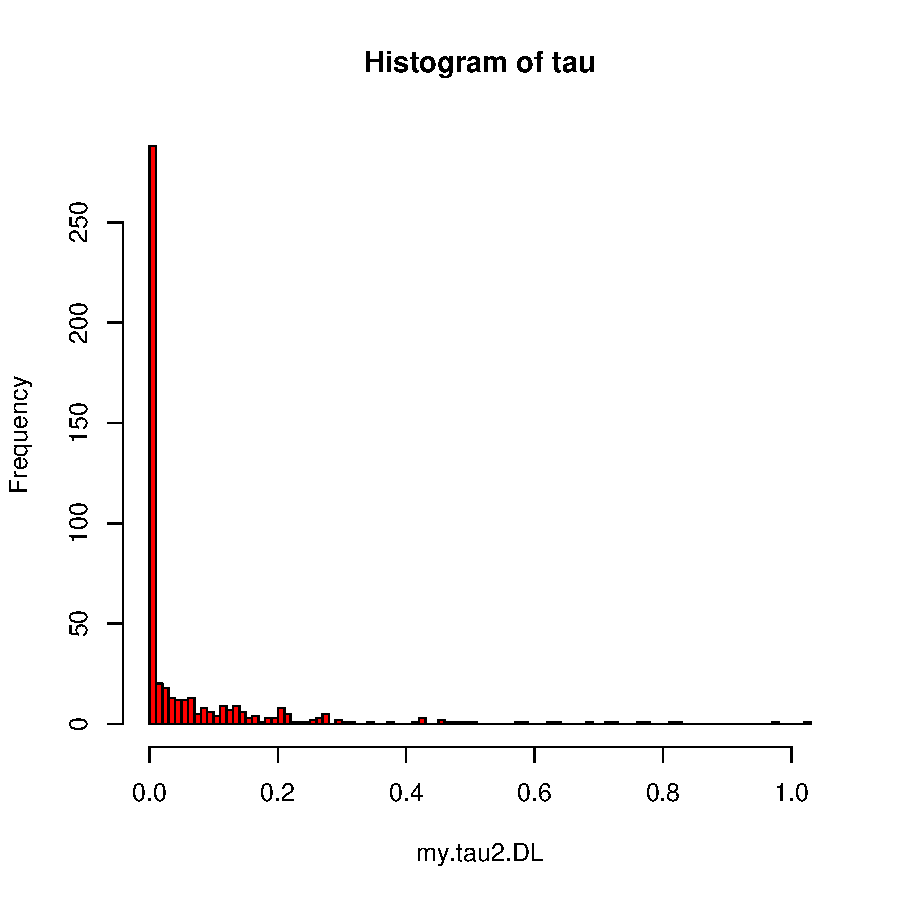
\includegraphics{MAMA_full-019}
\end{center}
\paragraph{Results}
The procedure described in details above is also implemented in function {\ttfamily zScores}. The arguments of this function are a list of expression sets ({\ttfamily esets}) and a list of classes ({\ttfamily classes}). Argument {\ttfamily useREM} chooses between REM and FEM. 
\begin{Schunk}
\begin{Sinput}
> esets <- GEDM(ColonData)
> classes <- selectClass(ColonData, "MSIstatus", "binary")
> theScores <- zScores(esets, classes, useREM = FALSE)
> round(theScores[1:2, ],3)
\end{Sinput}
\begin{Soutput}
            zSco_Ex_1 zSco_Ex_2 zSco_Ex_3   zSco MUvals
217562_at       2.091    -0.542     0.881  1.865  0.326
203766_s_at    -0.824    -0.085     0.855 -0.196 -0.034
            MUsds Qvals df Qpvalues Chisq Effect_Ex_1
217562_at   0.175 1.964  2    0.375 0.062       0.484
203766_s_at 0.174 1.379  2    0.502 0.845      -0.188
            Effect_Ex_2 Effect_Ex_3 EffectVar_Ex_1
217562_at        -0.262       0.283          0.053
203766_s_at      -0.041       0.275          0.052
            EffectVar_Ex_2 EffectVar_Ex_3
217562_at            0.233          0.103
203766_s_at          0.232          0.103
\end{Soutput}
\end{Schunk}
We get a matrix ({\ttfamily theScores}) with the following columns:
\begin{itemize}
\item \emph{Effect\_Ex\_ } are the unbiased estimates of the effect (\emph{d.adj. })
\item \emph{EffectVar\_Ex\_ } are the estimated variances of the unbiased effects (\emph{var.d.adj. })
\item \emph{zSco\_Ex\_} are the unbiased estimates of the effects divided by their standard deviation 
\item \emph{Qvals} are the Q statistics (\emph{my.Q}) and df is the number of combined experiments minus one
\item \emph{MUvals} and \emph{MUsds} are equal to \emph{muFEM} and \emph{sdFEM} (the overall mean effect size and its standard deviation) 
\item \emph{zSco} are the z scores (\emph{ZFEM})
\item \emph{Qpvalues} is for each gene the probability that a chi-square distribution with \emph{df} degree of freedom has a higher value than its $Q$ statistic
\item \emph{Chisq} is the probability that a chi-square distribution with 1 degree of freedom has a higher value than \emph{zSco2}
\end{itemize}
Function {\ttfamily zScoresFDR} implements SAM \cite{SAM} type analysis to estimate the false discovery rate (FDR). 
\begin{Schunk}
\begin{Sinput}
> ScoresFDR <- zScoreFDR(esets, classes, useREM = FALSE, nperm = 50, CombineExp = 1:3)
> names(ScoresFDR) 
\end{Sinput}
\begin{Soutput}
[1] "pos"       "neg"       "two.sided"
\end{Soutput}
\begin{Sinput}
> round(ScoresFDR$pos[1:2, ],3)
\end{Sinput}
\begin{Soutput}
            zSco_Ex_1 FDR_Ex_1 zSco_Ex_2 FDR_Ex_2 zSco_Ex_3
217562_at       2.091    0.083    -0.542    1.073     0.881
203766_s_at    -0.824    1.204    -0.085    1.006     0.855
            FDR_Ex_3   zSco   FDR MUvals MUsds Qvals df
217562_at      0.585  1.865 0.115  0.326 0.175 1.964  2
203766_s_at    0.585 -0.196 1.044 -0.034 0.174 1.379  2
            Qpvalues Chisq
217562_at      0.375 0.062
203766_s_at    0.502 0.845
\end{Soutput}
\end{Schunk}
Function {\ttfamily plotES} provides several visualizations of the results. Specifying {\ttfamily which=1} will plot so called \emph{IDRplot}. This plot shows the fraction of the genes that have a higher effect size than the threshold for the combined Z-score , but not for any of the data set specific Z-scores. Genes with combined Z-score $>0$ and $<0$ are plotted separately. Selection {\ttfamily which=2} will plot the number of genes and the corresponding FDR for the two sided situation. If the user is more interested in the number of genes that are below a given threshold for the FDR, one decides for {\ttfamily which=3}. It shows for each study (indicated by different colors) and various thresholds for the FDR (x axis) the number of genes that are below this threshold in the given study but above in all other studies are shown (y axis). If numeric vector is used that all figure specified in the vectors are plot. \par
Argument {\ttfamily legend.names} is a character vector with names of the date set used in legends and {\ttfamily colors} is a vector of colors to be used for plotting.
\begin{Schunk}
\begin{Sinput}
> plotES(theScores, ScoresFDR, num.studies=3, legend.names=c("Combined set",
+  "Denmark", "Australia", "Japan"), colors=c("red","blue",
+  "green","yellow"), which=1:3)
\end{Sinput}
\end{Schunk}
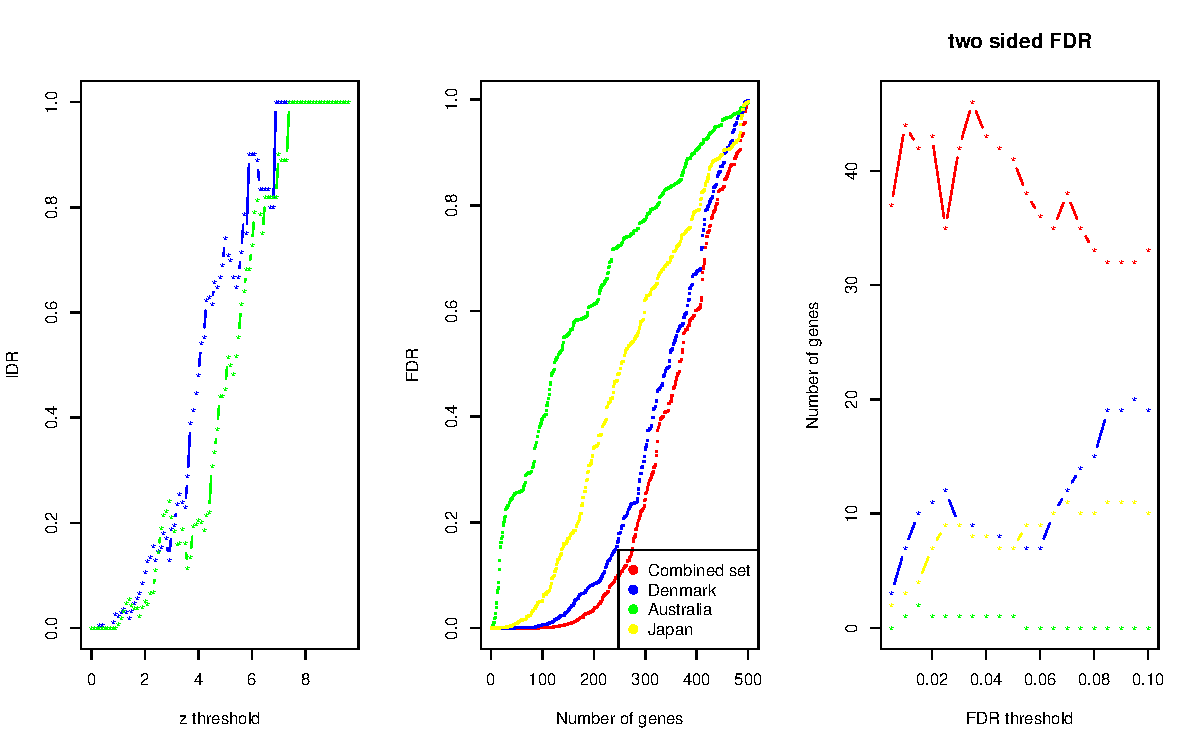
\includegraphics{MAMA_full-022}
\paragraph{Wrapper function}
There is also another function ({\ttfamily ES.GeneMeta}) that wrapes data preparation and functions {\ttfamily zScore}, {\ttfamily ScoresFDR}.
\begin{Schunk}
\begin{Sinput}
> es2<-ES.GeneMeta(ColonData, "MSIstatus", nperm = 100)
\end{Sinput}
\end{Schunk}
{\ttfamily nperm = 100} is used only for computational complexity. A thousand of permutation is more appropriate.  

\chapter{Similarity of Ordered Gene Lists (SOGL)}
%\addcontentsline{toc}{part}{Similarity of Ordered Gene Lists (SOGL)}
\section*{Introduction}
%\addcontentsline{toc}{section}{Introduction}
Similarity of Ordered Gene Lists is another method for meta-analysis of microarray. It is call as "comparison of comparisons" by its authors \cite{Yang2006}. \par
Briefly, it assigns a similarity score to a comparison of ranked (ordered) gene lists. The score is based on the number of overlapping genes in the top ranks. It computes the size of overlap for each rank. The final score is a weighted sum of these values, with more weight put on the top ranks. \par
\section*{Algorithm}
\begin{enumerate}
\item Required data sets - data sets with same set of genes are required. 
\item Ranking of genes - The genes are then ranked based on gene-wise test on difference of class mean. There is only one assumption about test result: a large positive test score corresponds to up-regulation and a large negative value to down-regulation. 
\item Computing the overlap - for each rank (from 1 to number of genes) we count the number of genes that appear in both ordered lists up to that position. It is denoted as $O_n(G_A,G_B)$, where $G_A$ and $G_B$ refer to ordered gene lists.
\item Similarity score - First we compute a total overlap $A_n$ at position $n$ given as $O_n(G_A,G_B)+O_n(f(G_A),f(G_B))$, where $f()$ means flipped list (down-regulated genes on top). Later we add weights to it and we sum it up to preliminary score. Weights $w_\alpha=e^{-\alpha.n}$ are used as default and tunning of parameter $\alpha$ is needed. The weights are used to put more importance on top genes. 

\end{enumerate}
The algorithm above is valid for meta-analysis in which expression data are not available. However, in this situation we can not use same approach for tunning $\alpha$. 
\section*{Usage}
%\addcontentsline{toc}{section}{Usage}
\subsection*{Data preparation}
As long as we have data stored in MetaArray object, there is no need for data transformation of any kind. We can move directly to order the genes as the first step in detecting differentially expressed genes.
\subsection*{Detecting differentially expressed genes}
Detection of diferentially expressed gene can be perfomed by a sequence of function or by one wrapper function. We will discuss both approaches below.\par
We start with ordering the genes from the most up-regulated to the most down-regulated ones. Function {\ttfamily computeOrdering} provides such functionality. It has three arguments: the dataset, name of clinical parameter with class labels and the test statistic (fold-change or t-test with unequal variance).
\begin{Schunk}
\begin{Sinput}
> ordering<- computeOrdering(ColonData, "MSIstatus", "T")
\end{Sinput}
\end{Schunk}
Now we have to tune the $\alpha$ parameter so we could obtain the similarity score.\par
Function {\ttfamily computeAlpha} returns vector of possible values for $\alpha$. These depend on the number of genes in analysis (argument {\ttfamily ngenes})or minimal weight (argument {\ttfamily min.weight}) to be considered in score calculation. One can also select a particular number of top genes to be analyzed (argument {\ttfamily n}). 
\begin{Schunk}
\begin{Sinput}
> A<-computeAlpha(ngenes=500)
> A
\end{Sinput}
\begin{Soutput}
[1] 0.11512925 0.07675284 0.05756463 0.03837642 0.02878231
[6] 0.02302585
\end{Soutput}
\end{Schunk}
When {\ttfamily n} is used only one value of $\alpha$ is returned.
\begin{Schunk}
\begin{Sinput}
> a<-computeAlpha(n=25, ngenes=500)
> a
\end{Sinput}
\begin{Soutput}
[1] 0.460517
\end{Soutput}
\end{Schunk}
Random permutation of class labels and subsampling are necessary to gather the optimal value for $\alpha$. This is the most computationaly complex step of the analysis. 
\begin{Schunk}
\begin{Sinput}
> random.score<-RandomScore(data = ColonData, varname = "MSIstatus", 
+ B = 10, alpha = A, test = "T",  two.sided = TRUE)
\end{Sinput}
\end{Schunk}
Function {\ttfamily RandomScore} performs random permutation of class labels and subsampling and returns a list with three slots. A matrix of smiliarity scores in which rows refer to $\alpha$'s and column to permutations is stored in \emph{random} slot. Similar results from subsampling are stored in \emph{subsample} slot. If {\ttfamily "empirical"}  is part of {\ttfamily which} argument then also 95\% empirical confidence intervals and medians of expected number of overlapping genes for each position are provided in \emph{empiricial.ci}. The argument {\ttfamily two.sided} is {\ttfamily TRUE} if both sides of ordered gene list are to be compared and {\ttfamily FALSE} if only top genes have to be considered.\par
Now, optimal value for $\alpha$ can be selected according to pAUC as a meassure of the separability of two distributions: scores after random permutation of class labels and scores after subsampling. The $\alpha$ with  the highest pAUC is selected.\par
\begin{Schunk}
\begin{Sinput}
> A.opt <- selectAlpha(A, random.score$subsample, random.score$random)
\end{Sinput}
\end{Schunk}
\subsection*{Results}
The final similarity score {\ttfamily score}, its significance {\ttfamily sig} and vector of genes which contribute to the overall similarity score {\ttfamily genes} can be obtained via:
\begin{Schunk}
\begin{Sinput}
> score<-prelimScore(ordering, A.opt$alpha)
> sig<-sigScore(ordering, A.opt$alpha, 100)
> genes<-selectGenes(ordering, A.opt$alpha, 0.95)
\end{Sinput}
\end{Schunk}
\subsection*{Wrapper function}
Function {\ttfamily performSOGL} is a wrapper function for Similarity of Ordered Gene Lists. 
\begin{Schunk}
\begin{Sinput}
> SOGL.res <- performSOGL(ColonData, varname = "MSIstatus", test = "FCH", 
+ B = 100, which=c("score", "empirical"), min.weight = 1e-05, two.sided = TRUE )
\end{Sinput}
\begin{Soutput}
Processing data...Tuning alpha..Significance and genes...
\end{Soutput}
\end{Schunk}
{\ttfamily SOGL.res} is a list that contains:
\begin{itemize}
\item \emph{ordering} ordered gene lists as a data.frame where columns refer to datasets
\item \emph{alpha.selected} selected value of alpha parameter 
\item \emph{alpha.considered} vector of alpha considered for selection
\item \emph{pAUC} pAUC values related to all alphas considered
\item \emph{random} random scores (permutations of class labels)
\item \emph{subsample} scores after subsampling from each class and dataset
\item \emph{emp.ci} empirical confidence intervals for number of overlapping genes
\item \emph{common.genes} vector of number of overlapping genes
\item \emph{score} observed similarity score
\item \emph{significance} significance of the observed score in form of p-value
\item \emph{genes} genes that account for observed similarity score
\end{itemize}

The {\ttfamily SOGL.res} is an object of class {\ttfamily SOGLresult} for which plot function exist. 
\begin{Schunk}
\begin{Sinput}
> par(mfrow = c(1, 3))
> plot(SOGL.res, "alpha selection")
> plot(SOGL.res, "density")
> plot(SOGL.res, "empirical CI")
\end{Sinput}
\end{Schunk}
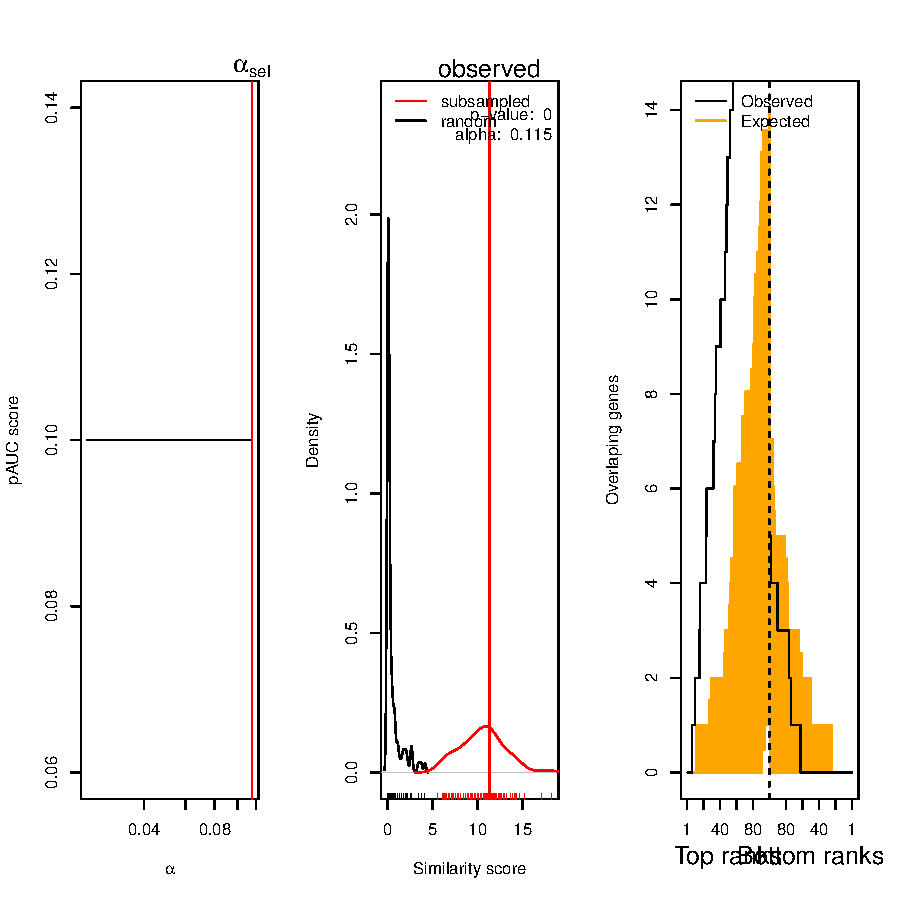
\includegraphics{MAMA_full-031}
The left graph shows pAUC of all $\alpha$'s considered. The selected $\alpha$ is singed by red vertical line. \par
In the center, one can see estimated densities of random (in black) and subsampled score (in red) for selected $\alpha$. The observed similarity score is marked by vertical line. The bottom rugs are scores actually achieved in permutations. 
The right graph displays the empirical confidence intervals for number of overlapping genes to each position. Obsereved overlaps are drawn as black step-function.




\chapter{RankProduct}
%\addcontentsline{toc}{part}{RankProduct}
\section*{Introduction}
%\addcontentsline{toc}{section}{Introduction}
RankProduct is a non-parametric statistic that detects up-regulated and down-regulated genes under one condition against another condition. In our sample data set we look for difference in expression between MSI and MSS colon cancer. \par
It focuses on genes which are consistently highly ranked in a number of lists, for example genes that are regularly found among top up-regulated genes in many microarray studies. It assumes that under the null hypothesis the order of all items is random then the probability of finding a certain item among the top $r$ of $n$ items in a list is $p=r/n$. Rank product is defined by multiplying these probabilities $RP=\prod_{i}\frac{r_i}{n_i}$, where $r_i$ is the rank of the item in the $i$-th list and $n_i$ is the total number of the items on $i$-th list. The smaller the $RP$ value the smaller the probability that the observation of the item at the top of the lists is due to chance. It is equivalent to calculating the geometric mean rank. A list of up- or down-regulated genes are selected based on the estimated percentage of false positive prediction (pfp) - known as false discovery rate (FDR), too.
\section*{Algorithm}
Algorithm of the method has five steps:
\begin{enumerate}
\item Fold-change ratio is calculated in each data set.
\item Ranks are assigned (1 for the highest value) according to fold-change ratio. $r_{gi}$ is rank of gene $g$ in comparison $i$, where $i$ is from $1$ to $K$, where $K$ is sum of products of number of slides in groups.
\item RankProduct for a gene ($RP_g$) is calculated as $\prod_{i}r_{gi}^{1/K}$
\item $l$ permutations of expression values at each microarray slide is performed and all previous steps repeated. We obtain $RP_g^{(l)}$
\item Step 4 is repeated $L$ times to estimate the distribution of $RP_g^{(l)}$. This distribution is used to calculate p-value and pfp for each gene.
\end{enumerate}
\section*{Usage}
This section depends on the {\ttfamily RankProd} package, which is free only for non-commercial users. Non-academic users MUST confirm with the authors. 
\begin{Schunk}
\begin{Sinput}
> library(RankProd)
\end{Sinput}
\end{Schunk}

\subsection*{Data preparation}
In order to run a rank product meta-analysis, user needs to call function {\ttfamily RPadvance}. It  requires three arguments: {\ttfamily data}, {\ttfamily cl} and {\ttfamily origin}. The first one {\ttfamily data} is the matrix (or data frame) containing the gene expression data that should be analyzed. Each of its rows corresponds to a gene, and each column corresponds to a sample. Second and third argument, {\ttfamily cl} and {\ttfamily origin}, are vectors of length {\ttfamily ncol(data)} containing the class labels of the samples or the origin labels of the samples. Function {\ttfamily mergedata} returns a list with three slots corresponding to arguments described above. {\ttfamily varname} argument is a string indicating which columns of the clinical data matrices should be used as class labels. 
\begin{Schunk}
\begin{Sinput}
> rankdata<-mergedata(ColonData, "MSIstatus")
> rankdata$cl
\end{Sinput}
\begin{Soutput}
  [1] 1 1 1 1 1 1 1 1 1 1 1 1 1 1 1 1 1 1 1 1 1 1 1 1 1 1 1
 [28] 1 1 1 1 1 1 1 1 1 1 1 1 2 2 2 2 2 2 2 2 2 2 2 2 2 2 2
 [55] 2 2 2 2 2 2 2 2 2 2 2 2 2 2 2 2 2 2 2 2 2 2 2 1 1 1 1
 [82] 1 2 2 2 2 2 2 2 2 2 2 2 2 2 2 2 2 2 2 2 2 2 2 2 2 2 2
[109] 2 2 2 2 2 1 1 1 1 1 1 1 1 1 1 1 1 1 1 1 1 2 2 2 2 2 2
[136] 2 2 2 2 2 2 2 2 2 2 2 2 2 2 2 2 2 2 2
\end{Soutput}
\begin{Sinput}
> rankdata$origin
\end{Sinput}
\begin{Soutput}
  [1] 1 1 1 1 1 1 1 1 1 1 1 1 1 1 1 1 1 1 1 1 1 1 1 1 1 1 1
 [28] 1 1 1 1 1 1 1 1 1 1 1 1 1 1 1 1 1 1 1 1 1 1 1 1 1 1 1
 [55] 1 1 1 1 1 1 1 1 1 1 1 1 1 1 1 1 1 1 1 1 1 1 1 2 2 2 2
 [82] 2 2 2 2 2 2 2 2 2 2 2 2 2 2 2 2 2 2 2 2 2 2 2 2 2 2 2
[109] 2 2 2 2 2 3 3 3 3 3 3 3 3 3 3 3 3 3 3 3 3 3 3 3 3 3 3
[136] 3 3 3 3 3 3 3 3 3 3 3 3 3 3 3 3 3 3 3
\end{Soutput}
\end{Schunk}
In {\ttfamily cl} all $1$'s refer to MSI samples and all $2$'s to MSS samples. Similarly in {\ttfamily origin}, $1$ belongs to samples from first data set ({\ttfamily denmark}), $2$ from second data set ({\ttfamily australia}) and $3$ from {\ttfamily japan} study. You can choose different numbers for labels, but same numbers are always treated like same samples from same class or with same origin.
\subsection*{Detecting differentially expressed genes}
In this section, we show how the rank product method can be applied to detect differentially expressed gene in our data sets in sence of meta-analysis. It means we will get two separate lists (up- and down-regulated genes separately) not two such lists for each data set. For each gene, one pfp (percentage of false prediction) is computed and used to select significant genes.
We can run meta-analysis by
\begin{Schunk}
\begin{Sinput}
> RP.out<-RPadvance(rankdata$dat,rankdata$cl,rankdata$origin,num.perm=10,
+ logged=TRUE,na.rm=FALSE,gene.names=rownames(GEDM(ColonData)[[1]]), plot=FALSE)
\end{Sinput}
\begin{Soutput}
 The data is from  3 different origins 
 
Rank Product analysis for two-class case 
 
Warning: Expected classlabels are 0 and 1. cl will thus be set to 0 and 1. 
 
Starting  10 permutations... 
Computing pfp... 
\end{Soutput}
\end{Schunk}
The data are log-transformed, therefore we set {\ttfamily logged=TRUE}. The number of permutations is default set to 100, you can change it to higher number, if you wish more precise estimates of the pfp. The argument {\ttfamily plot=FALSE} will prevent the graphical display of the estimated pfp vs. number of identified genes. We will use function {\ttfamily plotRP} for a such display.
\subsection*{Results}
\begin{center}
\begin{Schunk}
\begin{Sinput}
> plotRP(RP.out, cutoff=0.05)
\end{Sinput}
\end{Schunk}
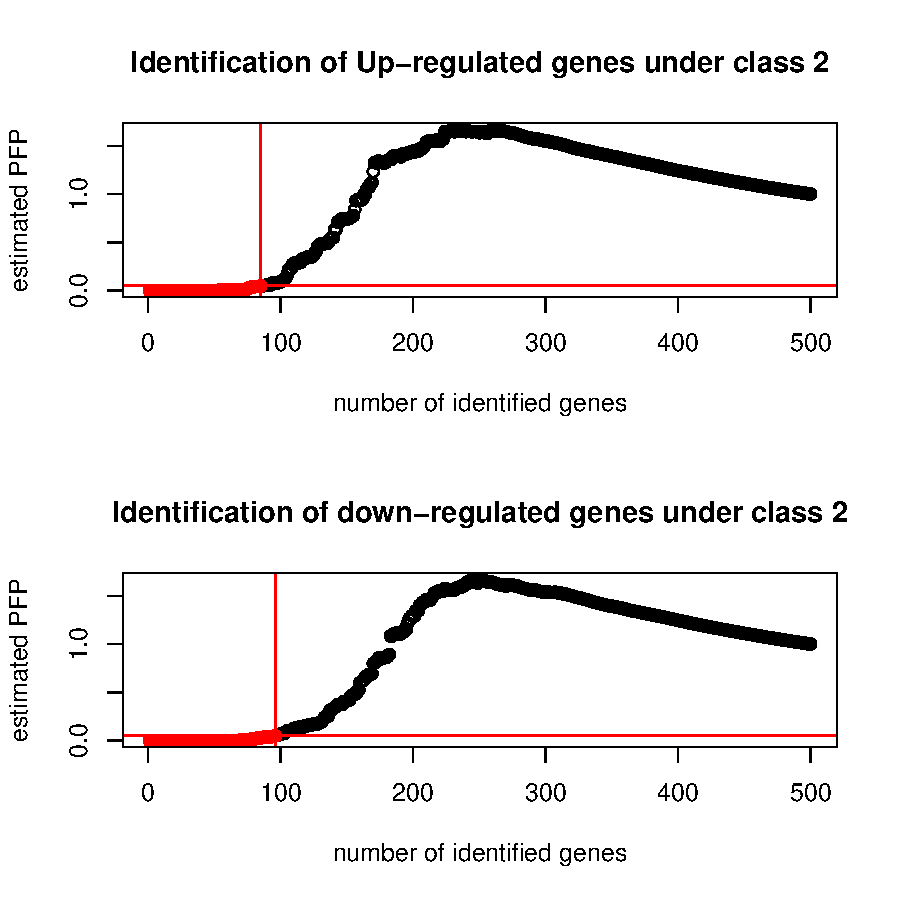
\includegraphics{MAMA_full-035}
\end{center}
The function {\ttfamily plotRP} graphicaly displays the estimated pfp vs. number of identified genes using the output from {\ttfamily RPadvance}. If cutoff (the maximum accepted pfp) is specified, identified genes are marked in red.
\begin{Schunk}
\begin{Sinput}
> RankRes<-topGene(RP.out, cutoff=0.05)
\end{Sinput}
\begin{Soutput}
Table1: Genes called significant under class1 < class2 

Table2: Genes called significant under class1 > class2 
\end{Soutput}
\begin{Sinput}
> head(round(RankRes$Table1,3))
\end{Sinput}
\begin{Soutput}
            gene.index RP/Rsum FC:(class1/class2) pfp
228030_at          254  15.955              0.234   0
228915_at          462  26.810              0.407   0
206239_s_at         77  28.268              0.344   0
243669_s_at        237  30.786              0.465   0
213880_at          258  40.144              0.520   0
213385_at          213  43.146              0.456   0
            P.value
228030_at         0
228915_at         0
206239_s_at       0
243669_s_at       0
213880_at         0
213385_at         0
\end{Soutput}
\begin{Sinput}
> head(round(RankRes$Table2,3))
\end{Sinput}
\begin{Soutput}
          gene.index RP/Rsum FC:(class1/class2) pfp P.value
205242_at        257  31.645              3.092   0       0
37145_at         154  34.843              2.678   0       0
209301_at        164  37.957              2.276   0       0
206442_at        280  42.928              2.927   0       0
206391_at        168  49.136              1.836   0       0
204818_at        277  50.370              2.216   0       0
\end{Soutput}
\end{Schunk}
The function {\ttfamily topGene} is used to output a table of the identified genes from the {\ttfamily RP.out}. Table contains genes according to other arguments. It is obligatory to specify either the {\ttfamily cutoff} (the desired significance of the identification) or {\ttfamily num.gene} (the number of top genes identified), otherwise a error message will be printed and the function will be stopped. If cutoff is selected, user needs to choose between {\ttfamily pfp} (percentage of false prediction) or {\ttfamily pval} (p-value). {\ttfamily pfp} is the default setting, which is selected when no selection is made.\par
Two tables are output, listing identified up- (Table1: class 1 < class 2) and down- (Table2: class1 > class 2) regulated genes. There are 5 columns in the table 
\begin{enumerate}
\item \emph{gene.index} is the gene index in the original data set
\item \emph{RP/Rsum} is the computed rank product for each gene
\item \emph{FC:(class1/class2)} is the computed fold change of the average expression levels under two conditions, which would be converted to the original scale using input logbase (default value is 2) if {\ttfamily logged=TRUE} is specified
\item \emph{pfp} is the estimated pfp value for each gene in the list if that gene serves as the cutoff point
\item \emph{P.value} is the associated P-values for each gene
\end{enumerate}

\subsection*{Wrapper function}
Function {\ttfamily RankProduct} needs no data preparation and provides the tables of identified up- and down- regulated genes.
\begin{Schunk}
\begin{Sinput}
> rp <- RankProduct(ColonData, "MSIstatus", num.perm = 10)
\end{Sinput}
\begin{Soutput}
 The data is from  3 different origins 
 
Rank Product analysis for two-class case 
 
Starting  10 permutations... 
Computing pfp... 
Table1: Genes called significant under class1 < class2 

Table2: Genes called significant under class1 > class2 
\end{Soutput}
\end{Schunk}

\chapter{Z-statistic - posterior mean differential expression}
%\addcontentsline{toc}{part}{Z-statistic - posterior mean differential expression}
\section*{Introduction}
%\addcontentsline{toc}{section}{Introduction}
The main idea of this method is that one can use data from one study to construct a prior distribution of differential expression and thus utilize the posterior mean differential expression, weighted by variances, whose distribution is standard normal distribution due to classic Bayesian probability calculation. \par
It is based on assumption that gene expression is normally distributed with mean $\mu_g $ and SD $\sigma^2_g$ and that we can estimate $\sigma^2_g$ by pooling together all genes with similar levels of mean intensity. The difference in gene expression is tested by
\[ Z=\frac{D}{\sigma_D}=\frac{\overline{X}_1 - \overline{X}_2}{\sqrt{\frac{\sigma_1^2}{n_1}+\frac{\sigma_2^2}{n_2}}} \sim N(0,1),\]
where $\overline{X}_1$ and $\overline{X}_2$ denotes mean gene expression values in classes, $\sigma_1^2$ and $\sigma_2^2$ denotes the estimated SD in classes and $n_1$ and $n_2$ denotes the number of samples in classes. 
\section*{Usage}
%\addcontentsline{toc}{section}{Usage}
\subsection*{Data preparation}
Because the same number of samples in each class and study is used in primary publication of the method \cite{Wang}, we will first look at number of samples in our data.
\begin{Schunk}
\begin{Sinput}
> ColonData
\end{Sinput}
\begin{Soutput}
Dataset Denmark  containing 500 probes and  77 samples. 
Sumarization of samples: 
MSIstatus 
--------- 
MSI MSS 
 39  38 
age 
--- 
   Min. 1st Qu.  Median    Mean 3rd Qu.    Max. 
  36.00   45.00   54.00   54.92   62.00   80.00 

Dataset Australia  containing 500 probes and  36 samples. 
Sumarization of samples: 
MSIstatus 
--------- 
MSI MSS 
  5  31 
age 
--- 
   Min. 1st Qu.  Median    Mean 3rd Qu.    Max. 
  50.00   57.75   66.00   66.36   73.75   85.00 

Dataset Japan  containing 500 probes and  41 samples. 
Sumarization of samples: 
location 
-------- 
  distal proximal  unknown 
      28       11        2 
MSIstatus 
--------- 
MSI MSS 
 16  25 
age 
--- 
   Min. 1st Qu.  Median    Mean 3rd Qu.    Max. 
  40.00   47.00   53.00   53.61   60.00   65.00 
\end{Soutput}
\end{Schunk}
The smallest value in the tables above is 5, therefore we will randomly choose 5 samples in each class and data set. Function {\ttfamily posterior.mean} performs such data reduction and Z-statistic calculation. It has three required arguments: a data set as MetaArray object ({\ttfamily data}), name of clinical parameter with class labels ({\ttfamily  varname}) and number of samples to be selected ({\ttfamily nsamp}). 
\subsection*{Detecting differentially expressed genes}
We apply this method by
\begin{Schunk}
\begin{Sinput}
> z.stat<-posterior.mean(ColonData, "MSIstatus", 5)
\end{Sinput}
\begin{Soutput}
0 marked as 0
1 marked as 1
Contrast will be 1 - 0 
\end{Soutput}
\end{Schunk}
\subsection*{Results}
\begin{Schunk}
\begin{Sinput}
> head(round(z.stat,3))
\end{Sinput}
\begin{Soutput}
             Zscore Pvalue
1552281_at    3.483  0.000
1552365_at   -4.342  0.000
1552485_at   -2.926  0.003
1552502_s_at -0.984  0.325
1552546_a_at -0.483  0.629
1552553_a_at -1.012  0.311
\end{Soutput}
\end{Schunk}
Only values of Z-statistic ({\ttfamily Zscore}) and their p-values ({\ttfamily Pvalue}) are outputs from this method.
\section*{Notes and discussion}
%\addcontentsline{toc}{section}{Notes and discussion}
This implementation expects either same microarray platform or same scale of expression values (like after POE transformation \cite{metaArray}) in all data sets.

          
\chapter{VennMapping}
%\addcontentsline{toc}{part}{VennMapping}
\section*{Introduction}
%\addcontentsline{toc}{section}{Introduction}
VennMapping \cite{Smid} is a method based on Venn diagrams and contingency tables. It looks for number of common genes in pairs of gene lists, statistical significance of observed match and returns also names of the common genes.
\section*{Algorithm}
%\addcontentsline{toc}{section}{Algorithm}
Algorithm of this method consists of three steps:
\begin{enumerate}
\item Calculation of fold-change in each data set.
\item Selection of significant (interesting) genes.
\item Comparison of gene lists pairs.
\end{enumerate}

\section*{Usage}
%\addcontentsline{toc}{section}{Usage}
\subsection*{Data preparation}
Function {\ttfamily fold.change} calculates mean fold-change in MetaArray object. It has two arguments: data set (e.g. {\ttfamily ColonData}) and name of the column with class labels to be used (e.g. {\ttfamily "MSIstatus"}). It assumes data are on $log_2$ scale.
\begin{Schunk}
\begin{Sinput}
> fc<-fold.change(ColonData, "MSIstatus")
\end{Sinput}
\end{Schunk}
Function {\ttfamily gene.select.FC} selects significant/interesting genes from mean fold-change matrix with rows referring  to genes and columns to data sets. The user has to specify (apart from mean fold-change matrix) a cutoff for selection. The cutoff is on $log_2$ scale, too. We chose $1$ for genes with at least 2-fold change in expression.
\begin{Schunk}
\begin{Sinput}
> list<-gene.select.FC(fc,1)
> summary(list)
\end{Sinput}
\begin{Soutput}
          Length Class  Mode     
Denmark   33     -none- character
Australia 27     -none- character
Japan     35     -none- character
\end{Soutput}
\end{Schunk}
Object {\ttfamily list} is a list in which each slot contains names of selected genes in one study. For example from the print above 33 genes have been selected in {\ttfamily denmark} data set. 
\subsection*{Detecting differentially expressed genes}
Now, we can move on comparison of selected gene lists in pairs of data sets. There are three functions to perform such a analysis: {\ttfamily conting.tab}, {\ttfamily Z} and {\ttfamily gene.list}. {\ttfamily conting.tab} returns contingency table with number of common genes. {\ttfamily Z} provides Z statistic to measure significance of observed number of common genes and {\ttfamily gene.list} outputs table with names of common genes. All of them have one argument same - it is a list object with names of selected genes in individual data sets. For function {\ttfamily Z} one additional argument is necessary - the number of genes involved in meta-analysis. 
\begin{Schunk}
\begin{Sinput}
> conting.tab(list)
\end{Sinput}
\begin{Soutput}
          Denmark Australia Japan
Denmark        NA        12    16
Australia      12        NA     7
Japan          16         7    NA
\end{Soutput}
\begin{Sinput}
> Z(list, n = 500)
\end{Sinput}
\begin{Soutput}
           Denmark Australia    Japan
Denmark         NA  7.920245 9.320174
Australia 7.869850        NA 3.821593
Japan     9.340196  3.854327       NA
\end{Soutput}
\begin{Sinput}
> gene.list(list)
\end{Sinput}
\begin{Soutput}
          Denmark                                                                                                                                                                 
Denmark   NA                                                                                                                                                                      
Australia "205009_at;206239_s_at;37145_at;205044_at;213385_at;228030_at;205242_at;204818_at;206442_at;202917_s_at;202589_at;230793_at"                                            
Japan     "202803_s_at;230964_at;213915_at;206239_s_at;1556055_at;1552281_at;37145_at;209301_at;206391_at;230621_at;243669_s_at;228030_at;206442_at;209436_at;230793_at;228915_at"
          Australia                                                                                                                   
Denmark   "205009_at;206239_s_at;37145_at;205044_at;213385_at;228030_at;205242_at;204818_at;206442_at;202917_s_at;202589_at;230793_at"
Australia NA                                                                                                                          
Japan     "206239_s_at;209583_s_at;37145_at;228030_at;206442_at;210143_at;230793_at"                                                  
          Japan                                                                                                                                                                   
Denmark   "202803_s_at;230964_at;213915_at;206239_s_at;1556055_at;1552281_at;37145_at;209301_at;206391_at;230621_at;243669_s_at;228030_at;206442_at;209436_at;230793_at;228915_at"
Australia "206239_s_at;209583_s_at;37145_at;228030_at;206442_at;210143_at;230793_at"                                                                                              
Japan     NA                                                                                                                                                                      
\end{Soutput}
\end{Schunk}
\subsection*{Wrapper function}
Function {\ttfamily VennMapper} provides both gene selection in each dataset and all comparisons of selected gene lists. 
\begin{Schunk}
\begin{Sinput}
> vm <- VennMapper(ColonData, "MSIstatus", 1)
> vm
\end{Sinput}
\begin{Soutput}
$conting.tab
          Denmark Australia Japan
Denmark        NA        12    16
Australia      12        NA     7
Japan          16         7    NA

$z.score
           Denmark Australia     Japan
Denmark         NA 14.964793 17.550323
Australia 14.93428        NA  8.098665
Japan     17.56230  8.120747        NA

$genes
          Denmark                                                                                                                                                                 
Denmark   NA                                                                                                                                                                      
Australia "205009_at;206239_s_at;37145_at;205044_at;213385_at;228030_at;205242_at;204818_at;206442_at;202917_s_at;202589_at;230793_at"                                            
Japan     "202803_s_at;230964_at;213915_at;206239_s_at;1556055_at;1552281_at;37145_at;209301_at;206391_at;230621_at;243669_s_at;228030_at;206442_at;209436_at;230793_at;228915_at"
          Australia                                                                                                                   
Denmark   "205009_at;206239_s_at;37145_at;205044_at;213385_at;228030_at;205242_at;204818_at;206442_at;202917_s_at;202589_at;230793_at"
Australia NA                                                                                                                          
Japan     "206239_s_at;209583_s_at;37145_at;228030_at;206442_at;210143_at;230793_at"                                                  
          Japan                                                                                                                                                                   
Denmark   "202803_s_at;230964_at;213915_at;206239_s_at;1556055_at;1552281_at;37145_at;209301_at;206391_at;230621_at;243669_s_at;228030_at;206442_at;209436_at;230793_at;228915_at"
Australia "206239_s_at;209583_s_at;37145_at;228030_at;206442_at;210143_at;230793_at"                                                                                              
Japan     NA                                                                                                                                                                      

attr(,"class")
[1] "VennMapper.res"
\end{Soutput}
\end{Schunk}

%\subsection*{Results}
%\section*{Discussion}
%\addcontentsline{toc}{section}{Discussion}

\chapter{MAP-Matches}
%\addcontentsline{toc}{part}{MAP-Matches}
\section*{Introduction}
%\addcontentsline{toc}{section}{Introduction}
Meta-Analysis Pattern Matches (MAP-Matches) \cite{Yang2005} is a method that extends VennMapping \cite{Smid} and meta-profiling \cite{velkyRhodes}. It is designed to analyze more distinct microarray data (search for common molecular mechanism in all types of cancer). It assumes same gene set in all data sets. 
\section*{Algorithm}
%\addcontentsline{toc}{section}{Algorithm}
Algorithm of this method has five steps:
\begin{enumerate}
\item Calculation of T-statistic for each two classes in each data set. 
\item Building matrix of T-statistics (T-matrix) with rows referring to genes and columns to pairs of classes and data set.
\item Selection of threshold for T-statistic.
\item Transformation of T-matrix into a binary matrix: 1 for T-statistics above threshold, 0 for T-statistics below threshold.
\item Statistical analysis of transformed T-matrix (more details in Usage section).  
\end{enumerate}

\section*{Usage}
%\addcontentsline{toc}{section}{Usage}
\subsection*{Data preparation}
The analysis starts with calculation of T-statistics. Function {\ttfamily meta.test} returns a list with two slots: matrix of test statistics ({\ttfamily test}) and matrix of p-values ({\ttfamily p}). In each of the matrices rows correspond to genes and columns to data sets. We need only {\ttfamily test} slot for this method. Argument {\ttfamily varname} is a string indicating which column of clinical data should be used as class labels. 
\begin{Schunk}
\begin{Sinput}
> stat.real<-meta.test(ColonData, varname = "MSIstatus")$test
\end{Sinput}
\end{Schunk}
\subsection*{Detecting differentially expressed genes}
The do not select significant genes in each study we only set threshold for T-statistics. We decided for 95 \% quantile (500 genes in 3 datasets with 95\% quantile leaves top 75 significance tests for the analysis). If there is a lot of genes and datasets in the meta-analysis one should consider higher quantiles. 
\begin{Schunk}
\begin{Sinput}
> stat <- c(stat.real)
> quan <- quantile(abs(stat), seq(0.00, 1.00, 0.0001))
> T.default <- quan["95.00%"]
\end{Sinput}
\end{Schunk}
Now, we transform {\ttfamily stat.real} (T-matrix) into a binary matrix. We replace T-statistics above threshold with $1$ and below with $0$.
\begin{Schunk}
\begin{Sinput}
> value.dis <- apply(stat.real,MARGIN=c(1,2), function(x) ifelse(abs(x)>T.default,1,0))
> rownames(value.dis)<-rownames(GEDM(ColonData)[[1]])
> head(value.dis)
\end{Sinput}
\begin{Soutput}
             Denmark Australia Japan
217562_at          0         0     0
203766_s_at        0         0     0
1554394_at         0         0     0
212662_at          0         0     0
1555370_a_at       0         0     0
240574_at          1         0     0
\end{Soutput}
\end{Schunk}
Each row {\ttfamily value.dis} is called a meta-analysis pattern. We are going to analyze their occurrence, significance and genes they occur at. Function {\ttfamily ratio} provides basic summarization of {\ttfamily value.dis}. 
\begin{Schunk}
\begin{Sinput}
> results<-ratio(value.dis)
> summary(results)
\end{Sinput}
\begin{Soutput}
         Length Class  Mode     
n         3     -none- numeric  
X.string 54     -none- character
p.strong  7     -none- numeric  
p.soft    7     -none- numeric  
\end{Soutput}
\end{Schunk}
In {\ttfamily results} we can find: number of genes with T-statistic sufficiently high in each study \emph{n}, patterns observed in data (\emph{X.String}), probability of observing strong match (\emph{p.strong}) and probability of observing soft match (\emph{p.soft}). We say two patterns match strongly if they are equal. The rule for soft match is weaker as only $1$'s in patterns must match. \par
Function {\ttfamily MAPmatrix} calculates a matrix with rows corresponding to patterns and four columns: unique patterns that are being observed in our data (\emph{uniqe.pat}), number of observed soft matches with the pattern (\emph{n.soft}), number of observed strong matches (\emph{n.strong} and number of $1$'s in the pattern \emph{n.sig}).
\begin{Schunk}
\begin{Sinput}
> MAPmat<-MAPmatrix(value.dis)
> MAPmat
\end{Sinput}
\begin{Soutput}
    unique.pat n.soft n.strong n.sig
100        100     38       22     1
110        110      7        4     2
010        010     15        6     1
101        101     12        9     2
001        001     22        8     1
011        011      5        2     2
111        111      3        3     3
\end{Soutput}
\end{Schunk}
Only pattern with multiply $1$'s are connected with common molecular mechanism and we will focus on them in the rest of analysis.
\begin{Schunk}
\begin{Sinput}
> MAPmat2<-MAPmat[MAPmat$n.sig>1,]
> unique.pat<-as.character(MAPmat2[,1])
\end{Sinput}
\end{Schunk}
We assume that sufficiently high number of strong matches may provides evidence of common molecular mechanism. Functions {\ttfamily MAPsig1} and {\ttfamily MAPsig2} perform statistical analysis to answer whether we observe significant number of matches or not. The statistical analysis can be done in two ways (both based on permutation testing): we either permute columns of T-matrix (in binary form) or permute class labels in data sets and repeat the whole procedure with same threshold for T-statistics. The former is implemented in {\ttfamily MAPsig1} and the latter in {\ttfamily MAPsig2}. Function {\ttfamily test.group.shuffle} calculates T-statistics with permuted class label repeatedly. 

\begin{Schunk}
\begin{Sinput}
> p1<-MAPsig1(unique.pat,value.dis,iter=100)
\end{Sinput}
\begin{Soutput}
Permutation: 
50 
100 
\end{Soutput}
\begin{Sinput}
> p1
\end{Sinput}
\begin{Soutput}
  p.soft p.strong
1      0     0.00
2      0     0.00
3      0     0.12
4      0     0.00
\end{Soutput}
\end{Schunk}
\begin{Schunk}
\begin{Sinput}
> out<-test.group.shuffle(ColonData, "MSIstatus", B = 100)
> p2 <- MAPsig2(out, value.dis, unique.pat, B = 100)
\end{Sinput}
\end{Schunk}
\begin{Schunk}
\begin{Sinput}
> p2
\end{Sinput}
\begin{Soutput}
  permu.soft permu.strong
1          0         0.03
2          0         0.00
3          0         0.17
4          0         0.00
\end{Soutput}
\end{Schunk}
Both \emph{p1} and \emph{p2} have same structure: rows refer to patterns and columns to statistical signifficance of observed soft (\emph{p.soft} or \emph{permu.soft}) or strong (\emph{p.strong} or \emph{permu.strong}) matches. 
\subsection*{Results}
Finally, we will bind all necessary outputs together. 
\begin{Schunk}
\begin{Sinput}
> resx <- cbind(MAPmat2, p1, p2)
> colnames(resx) <-c(colnames(MAPmat2), "p.strong", 
+ "p.weak", "p.permu.strong", "p.permu.weak")
> intx <- t(as.matrix(resx[which(resx[,4]<0.06),]))
> t(resx)
\end{Sinput}
\begin{Soutput}
               110    101    011    111   
unique.pat     "110"  "101"  "011"  "111" 
n.soft         " 7"   "12"   " 5"   " 3"  
n.strong       "4"    "9"    "2"    "3"   
n.sig          "2"    "2"    "2"    "3"   
p.strong       "0"    "0"    "0"    "0"   
p.weak         "0.00" "0.00" "0.12" "0.00"
p.permu.strong "0"    "0"    "0"    "0"   
p.permu.weak   "0.03" "0.00" "0.17" "0.00"
\end{Soutput}
\end{Schunk}
We can plot p-values by
\begin{center}
\begin{Schunk}
\begin{Sinput}
> plotpattern(resx, method=1)
\end{Sinput}
\end{Schunk}
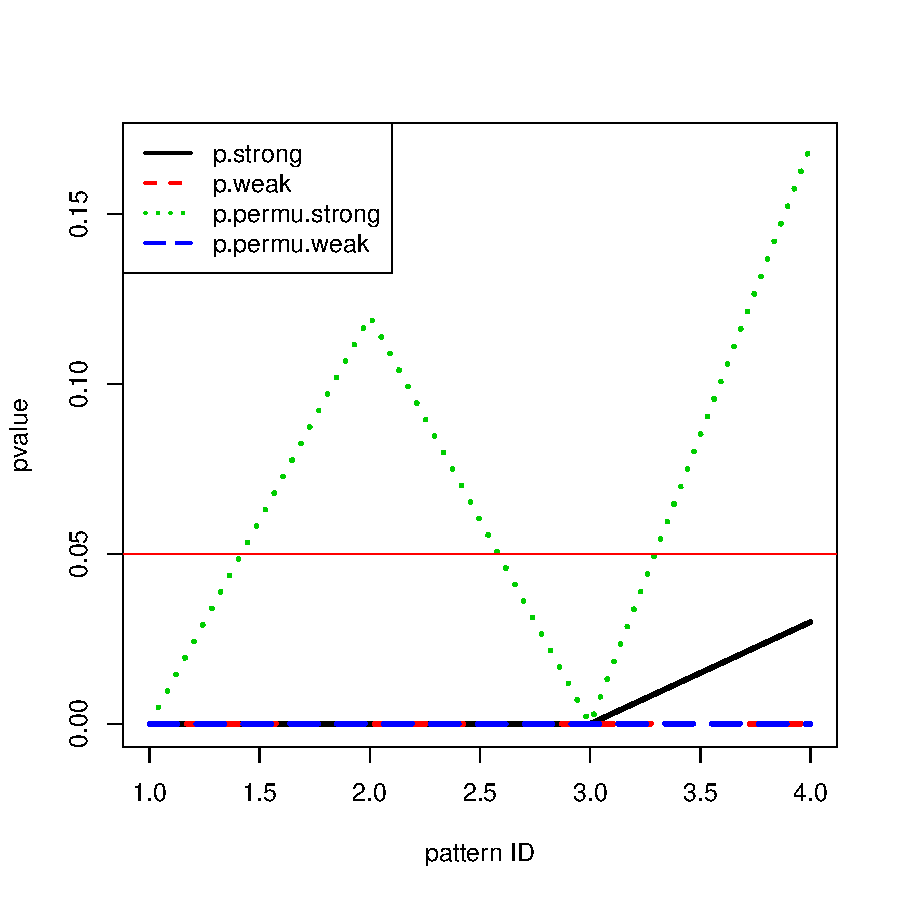
\includegraphics{MAMA_full-055}
\end{center}
or
\begin{center}
\begin{Schunk}
\begin{Sinput}
> plotpattern(resx, method=2)
\end{Sinput}
\end{Schunk}
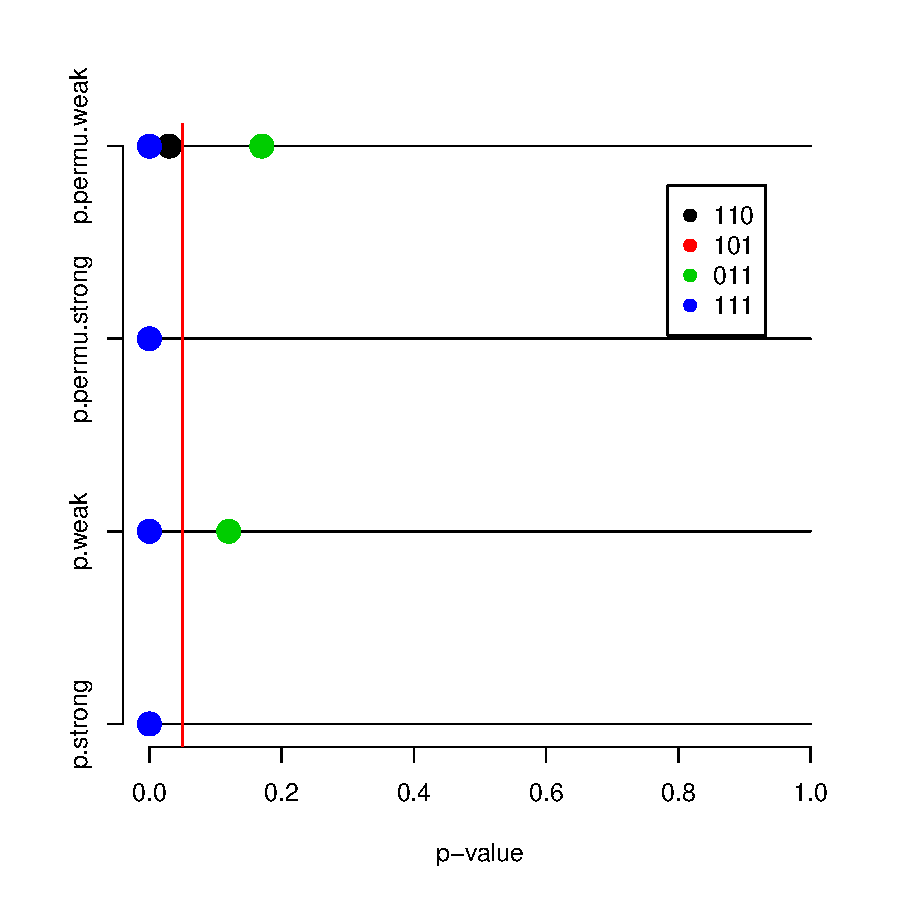
\includegraphics{MAMA_full-056}
\end{center}
Until now, we have only found out that for some patterns there is significantly high count of strong or soft matches being observed. Obviously we want to know expression of which genes is changed in these patterns. Function {\ttfamily MAP.genes} returns a list in which each slot contains list of genes involved in one pattern. If argument {\ttfamily files} is set to {\ttfamily TRUE} a files with gene names are also saved. 
\begin{Schunk}
\begin{Sinput}
> probs<-MAP.genes(resx,value.dis, files=FALSE)
> names(probs)<-rownames(resx)
> summary(probs)
\end{Sinput}
\begin{Soutput}
    Length Class  Mode     
110  7     -none- character
101 12     -none- character
011  5     -none- character
111  3     -none- character
\end{Soutput}
\end{Schunk}
\emph{probs} is a list with each slot referring to one pattern and list of gene names is stored there. The pattern has been observed at these genes.  
\par
\subsection*{Wrapper function}
Function {\ttfamily MAP.Matches} provides all steps of MAP-Matches method in one-line command. In
\begin{Schunk}
\begin{Sinput}
> map <- MAP.Matches(ColonData, "MSIstatus", 
+ t.cutoff = "95.00%", nperm = 100, sig.col = "p.col.strong")
\end{Sinput}
\begin{Soutput}
Examinig the data...
Statistical analysis...
Permutation: 
50 
100 
Permuting class labels in dataset: 
Denmark 
Australia 
Japan 
Permutation: 
50 
100 
\end{Soutput}
\end{Schunk}
the first argument is the dataset (MetaArray object), the second one is a column name of the class labels, {\ttfamily nperm} denotes the number of permutations and the last one {\ttfamily sig.col} is column name for selection of significant patterns - {\ttfamily "p.col.strong"} refer to the p-value of the strong matches when permutation of columns are used.
%\section*{Discussion}
%\addcontentsline{toc}{section}{Discussion}

\chapter{METRADISC}
%\addcontentsline{toc}{part}{METRADISC}
\section*{Introduction}
%\addcontentsline{toc}{section}{Introduction}
METRADISC \cite{Zintzaraz} is unique among rank-based methods because it provides an estimate of heterogeneity as one of its outputs. Additionally the method can deal with genes which are being measured in only some of the studies. The implementation available in MAMA package is restricted to genes common in all microarray studies analyzed.
\section*{Algorithm}
%\addcontentsline{toc}{section}{Algorithm}
\begin{enumerate}
\item Gene Ranking - In microarray analysis we usually test samples for a large number of genes. The results provide for each gene a test statistic and its statistical significance (p-value). Therefore we can rank the tested genes in each study based on direction in expression change and statistical significance. If there are $n$ genes being tested, the highest rank $n$ is given to the gene that shows the lowest $p$-value and it is up-regulated in diseased samples. Then follow all other up-regulated genes ranked according to increasing $p$-value. These are followed by down-regulated genes and the lowest rank ($1$) is given to gene that shows the lowest $p$-value and is down-regulated in diseased samples. Genes with equal $p$-values are assigned tied ranks. 
\item The Average Rank and Heterogeneity metrics - In this step we compute a average rank and heterogeneity metrics. The average rank $R^*$ is defined as $R^*= \frac{\sum_{i=1}^{s}R_i}{s}$, where $R_i$ is the rank of the gene in study $i$ and $s$ is total number of studies ($i=1,2,...,s$). The heterogeneity metrics $Q^*$ is given by formula $Q^*=\sum_{i=1}^{s}(R_i-R^*)^2$, it is actually generalization of Cochran's $Q$ statistic. 
\item Monte Carlo permutation test - To obtain statistical significance for average rank and heterogeneity metrics we randomly permute the ranks of each study and the stimulated metrics are calculated. Then we repeat the procedure to generate null distribution for the metrics. Each variable is then tested against the corresponding null distribution. We are interested genuinely in four statistical significances: for high average rank, for low average rank, for high heterogeneity and for low heterogeneity. Distinction between high and low average rank is important as we want to keep the direction of effect in mind. Ignoring it can lead to spurious results that a gene is consistently significant even if it is up-regulated in one study and down-regulated in second one. On the other hand, statistically low heterogeneity may suggest consistent results among different studies. The statistical significance for high average rank ($R^*$) is defined as the percentage of simulated metrics that exceed or are equal to the observed ($R^*$). The statistical significance for low average rank ($R^*$) is defined as the percentage of simulated metrics that are below or equal to the observed ($R^*$). Significance of heterogeneity is defined analogously.  
\end{enumerate}
\section*{Usage}
%\addcontentsline{toc}{section}{Usage}
\subsection*{Data preparation}
We will start with computing test statistic and p-value for each gene and data set. Function {\ttfamily meta.test} returns a list with two slots: data frame of test statistics and data frame of p-values. In each of the matrices rows correspond to genes and columns to data sets. Argument {\ttfamily varname} is a string indicating which column of clinical data should be used as class labels. 
\begin{Schunk}
\begin{Sinput}
> metra<-meta.test(ColonData, varname = "MSIstatus")
> head(metra$test)
\end{Sinput}
\begin{Soutput}
                Denmark  Australia      Japan
217562_at    -2.1666481  1.0669144 -0.9286918
203766_s_at   0.8318955  0.1014991 -0.9459710
1554394_at    1.2176000  4.0282590  1.1763280
212662_at     1.9755557  1.3046695  2.5983263
1555370_a_at  4.3678119 -0.6042763  2.7174563
240574_at     5.1746999  1.6404196  1.8830312
\end{Soutput}
\end{Schunk}
\subsection*{Detecting differentially expressed genes}
Now, we can proceed to ranking genes. Function {\ttfamily rank.genes.adv} ranks the genes as described in Algorithm section above. 
\begin{Schunk}
\begin{Sinput}
> RANK<-rank.genes.adv(metra)
> head(RANK)
\end{Sinput}
\begin{Soutput}
             Denmark Australia Japan
217562_at        105       368   156
203766_s_at      326       257   153
1554394_at       348       488   380
212662_at        390       397   442
1555370_a_at     473       170   445
240574_at        484       424   419
\end{Soutput}
\end{Schunk}
The genes ranks can be visualized by
\begin{center}
\begin{Schunk}
\begin{Sinput}
> RANK2<-RANK[order(RANK[,1]),]
> colnames(RANK2)<-c("Denmark","Australia", "Japan")
> heatcol<-colorRampPalette(c("Green", "Black", "Red"))(100)
> metaheat(as.matrix(RANK2), col=heatcol, c.cex = 0.8)
\end{Sinput}
\end{Schunk}
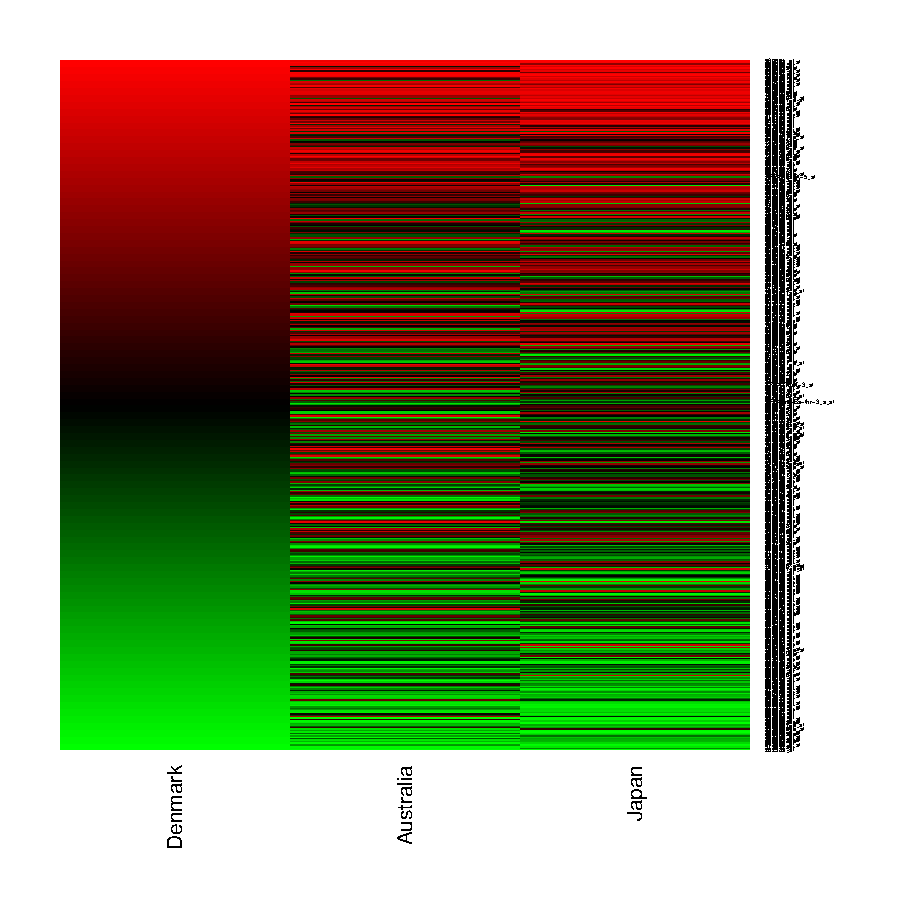
\includegraphics{MAMA_full-061}
\end{center}
The next step is to compute average rank $R^*$ and heterogeneity metric $Q^*$ for each gene.
\begin{Schunk}
\begin{Sinput}
> RQ<-compute.RQ(RANK)
> head(round(RQ,1))
\end{Sinput}
\begin{Soutput}
             r.star  q.star
217562_at     209.7 38904.7
203766_s_at   245.3 15168.7
1554394_at    405.3 10762.7
212662_at     409.7  1592.7
1555370_a_at  362.7 56072.7
240574_at     442.3  2616.7
\end{Soutput}
\end{Schunk}
And finally we use function {\ttfamily MCtest} to perform Monte Carlo permutation test. Function requires the observed ranks ({\ttfamily RANK}), observed average rank and heterogeneity metric ({\ttfamily RQ}) and number of permutations ({\ttfamily nper}) as arguments. Number of permutations depends on the required accuracy for the final $p$-values. $1/nper$ is the accuracy for the final $p$-values. For example with $1000$ permutations the $p$-values are calculated with three decimal places.  
\begin{Schunk}
\begin{Sinput}
> MC<-MCtest(RANK,RQ, nper=1000)
\end{Sinput}
\begin{Soutput}
100   200   300   400   500   600   700   800   900   1000   
\end{Soutput}
\begin{Sinput}
> head(MC)
\end{Sinput}
\begin{Soutput}
             R.high R.low Q.high Q.low
217562_at     0.667 0.333  0.468 0.532
203766_s_at   0.523 0.477  0.747 0.253
1554394_at    0.041 0.959  0.801 0.199
212662_at     0.033 0.967  0.950 0.050
1555370_a_at  0.080 0.920  0.303 0.697
240574_at     0.011 0.989  0.942 0.058
\end{Soutput}
\end{Schunk}
\subsection*{Results}
The command below creates a character vector of genes with significant average ranks and low heterogeneity. The selected threshold for statistical significance is $0.05$.
\begin{Schunk}
\begin{Sinput}
> METRA<-c(rownames(MC)[MC[,1]<0.05 & MC[,4]<0.05], 
+ rownames(MC)[MC[,2]<0.05 & MC[,4]<0.05])
> METRA[1:10]
\end{Sinput}
\begin{Soutput}
 [1] "239442_at"   "234207_at"   "225802_at"   "230964_at"  
 [5] "1563364_at"  "206239_s_at" "236223_s_at" "222551_s_at"
 [9] "1560119_at"  "201279_s_at"
\end{Soutput}
\end{Schunk}
\subsection*{Wrapper function}
Function {\ttfamily METRADISC} performs all steps of this method in one command.
\begin{Schunk}
\begin{Sinput}
> metra<-METRADISC(ColonData, "MSIstatus", nperm = 1000)
\end{Sinput}
\begin{Soutput}
100   200   300   400   500   600   700   800   900   1000   
\end{Soutput}
\begin{Sinput}
> str(metra)
\end{Sinput}
\begin{Soutput}
List of 3
 $ ranks :'data.frame':	500 obs. of  3 variables:
  ..$ Denmark  : num [1:500] 105 326 348 390 473 484 83 126 498 482 ...
  ..$ Australia: num [1:500] 368 257 488 397 170 424 179 187 490 495 ...
  ..$ Japan    : num [1:500] 156 153 380 442 445 419 88 187 390 469 ...
 $ RQ    : num [1:500, 1:2] 210 245 405 410 363 ...
  ..- attr(*, "dimnames")=List of 2
  .. ..$ : chr [1:500] "217562_at" "203766_s_at" "1554394_at" "212662_at" ...
  .. ..$ : chr [1:2] "r.star" "q.star"
 $ MCtest: num [1:500, 1:4] 0.683 0.524 0.031 0.024 0.111 0.006 0.934 0.845 0.002 0 ...
  ..- attr(*, "dimnames")=List of 2
  .. ..$ : chr [1:500] "217562_at" "203766_s_at" "1554394_at" "212662_at" ...
  .. ..$ : chr [1:4] "R.high" "R.low" "Q.high" "Q.low"
 - attr(*, "class")= chr "METRADISC.res"
\end{Soutput}
\end{Schunk}
It returns a list with ranks for each gene and dataset {\emph ranks}, average rank and heterogeneity for each gene {\emph RQ} and results of the Monte Carlo test {\emph MCtest}.
%\section*{Discussion}
%\addcontentsline{toc}{section}{Discussion}

\part{Results combination}
%\section{Methods comparison}
In this part we are going to compare and combine outputs from all methods so we can look and changes in gene expression in various ways. \par
We are going to start with lists of differentially expressed genes, because this is the only one output common for all methods mentioned in this vignette. We will merge all lists into one variable via function {\ttfamily join.DEG}. The function requires a complete list of genes involved in meta-analysis so it can map indices to gene names like for example function {\ttfamily pvalcombination} provides.  Because the same set of genes was measured in each data set we can arbitrarily choose one data set. 
\begin{Schunk}
\begin{Sinput}
> lists<-join.DEG(pvalt, ESt, ScoresFDR, SOGL.res, RankRes, z.stat, 
+  probs,genenames=rownames(GEDM(ColonData)[[1]]), 
+ type=c(1,1,3,4,5,6,7), cutoff=0.02)
> #or
> lists2<-join.DEG(pval, es, es2, SOGL.res, rp, z.stat, map,
+ genenames=rownames(GEDM(ColonData)[[1]]),  cutoff=0.05)
> names(lists)<-c("PvalCom", "ESCom","ESCom2","OrderedList","RankProduct", 
+ "Z-stat","MAP")
> summary(lists)
\end{Sinput}
\begin{Soutput}
            Length Class  Mode     
PvalCom     215    -none- character
ESCom       109    -none- character
ESCom2      178    -none- character
OrderedList  11    -none- character
RankProduct 178    -none- character
Z-stat      149    -none- character
MAP          18    -none- character
\end{Soutput}
\end{Schunk}
The argument {\ttfamily type} is a numeric identification of the method the object originates. When wrapper function are used there is no need for this argument.\par
Now, we will transform this list to a binary matrix where rows refer to genes and columns to method and $1$ means that the gene was identified as a differentially expressed gene in the method. Function {\ttfamily make.matrix} provides such transformation.  
\begin{Schunk}
\begin{Sinput}
> MAT<-make.matrix(lists)
> MAT[1:5,1:5]
\end{Sinput}
\begin{Soutput}
             PvalCom ESCom ESCom2 OrderedList RankProduct
1554394_at         1     0      0           0           0
212662_at          1     0      1           0           0
1555370_a_at       1     0      1           0           1
240574_at          1     1      1           0           1
203553_s_at        1     1      1           0           0
\end{Soutput}
\end{Schunk}
It is very popular to visualize results of microarray analysis as a heatmap. A heatmap is a graphical representation for a numeric matrix where values are presented as colors. Gene expression values are usually used in microarray analysis. In these pictures colors go continuously from green (for down-regulation) through black (for no change in gene expression) to red (for up-regulation). There are several R-packages which implement plotting heatmaps in slightly different way. Functions {\ttfamily metaheat} and {\ttfamily metaheat2} are modification of two of them, so a discrete set of colors (only two in {\ttfamily metaheat} but even several in {\ttfamily metaheat2}) can be used with an appropriate legend.\par
Function {\ttfamily metaheat} has three arguments: a data matrix ({\ttfamily MAT}), a number defining position of legend ({\ttfamily legend=1} is legend drawn below the picture) and vector of colors ({\ttfamily col}). 
\begin{center}
\begin{Schunk}
\begin{Sinput}
> metaheat(MAT, legend=1, col=c("red3", "royalblue2"))
\end{Sinput}
\end{Schunk}
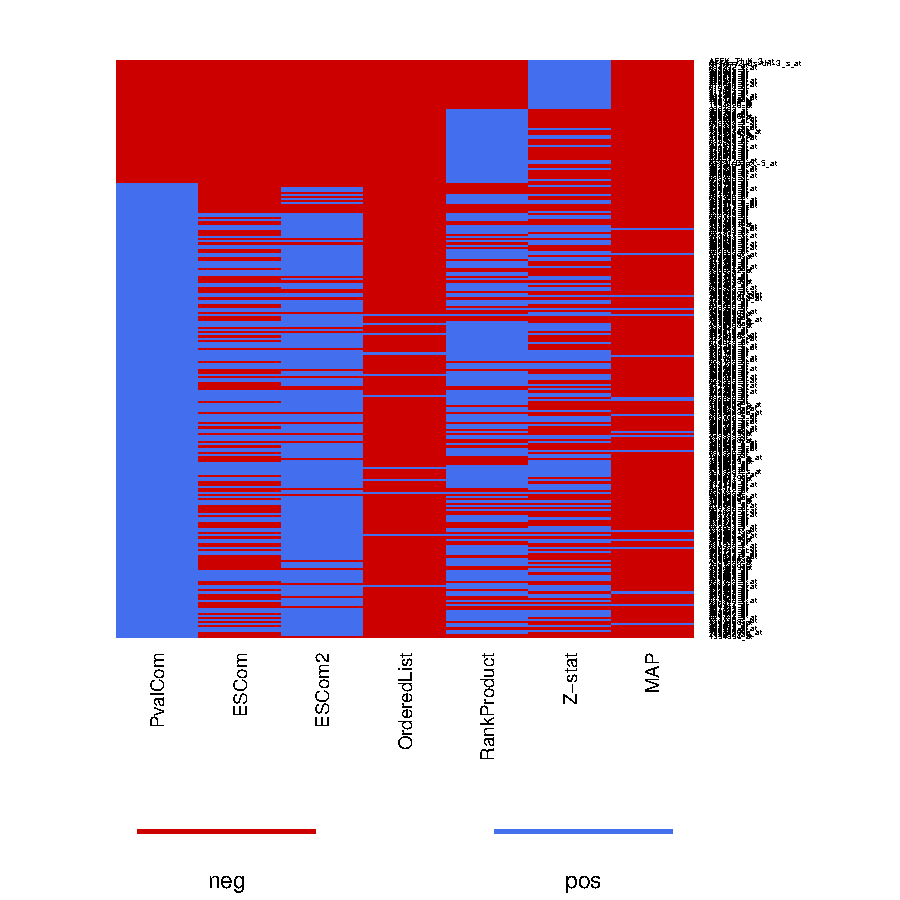
\includegraphics{MAMA_full-068}
\end{center}                  
 Function {\ttfamily metaheat2} has as many arguments as {\ttfamily heatmap.2} form gplots package and two more. Argument {\ttfamily legend.names} is a character vector with labels to be used in legend. Setting {\ttfamily discret=TRUE} will indicate that legend for discrete values should be drawn. 
\begin{center}
\begin{Schunk}
\begin{Sinput}
> metaheat2(MAT, col=c("red3", "royalblue2"), legend.names=c("DEG","noDEG"), 
+ discrete=TRUE, trace="none", dendrogram="none")
\end{Sinput}
\end{Schunk}
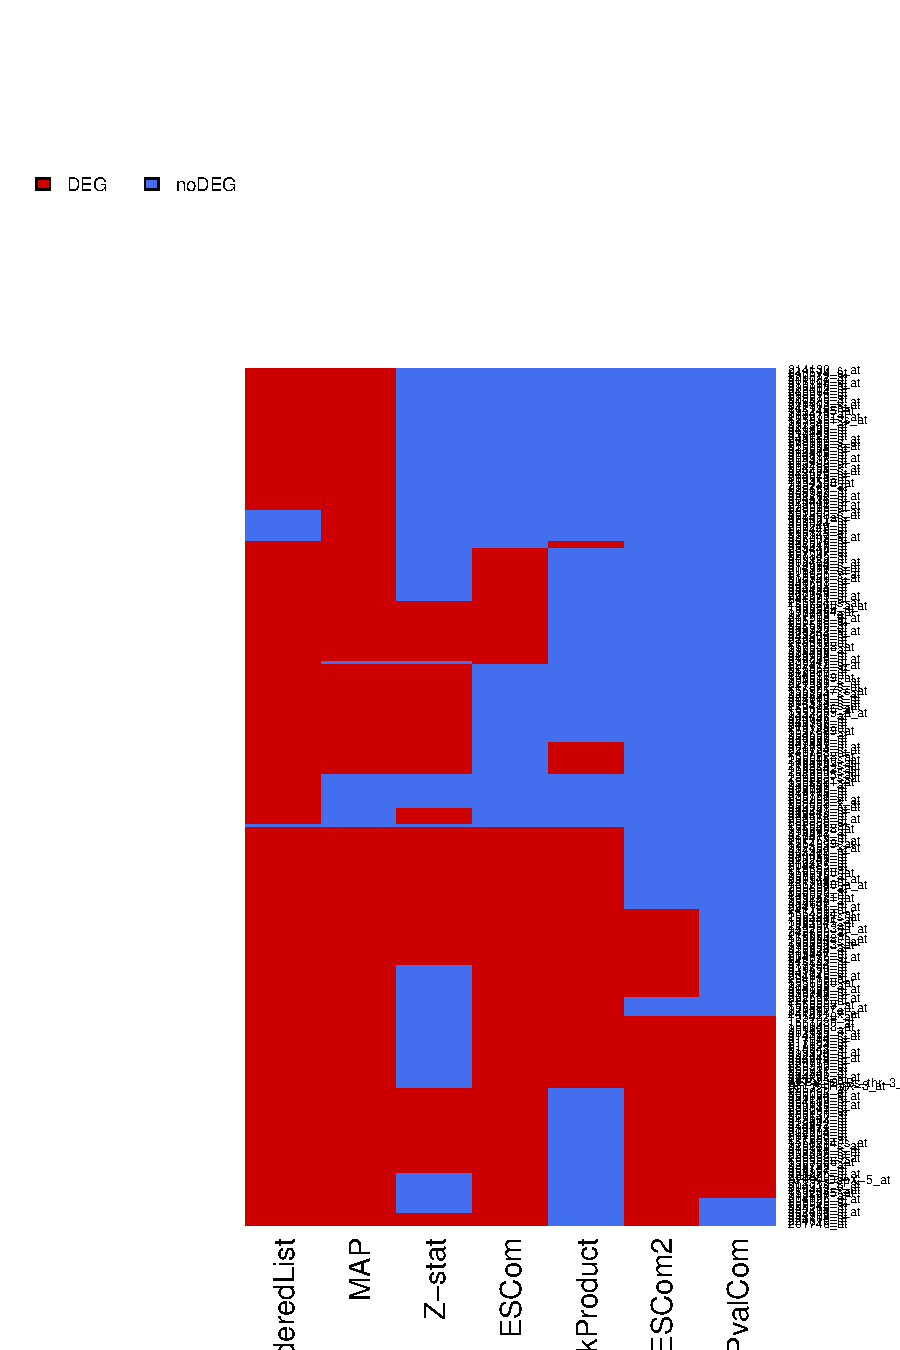
\includegraphics{MAMA_full-069}
\end{center}
The user can perform cluster analysis on {\ttfamily MAT} to search for similarities between methods or genes.\par
We can look at number of genes found by number of methods by
\begin{Schunk}
\begin{Sinput}
> dim(MAT)
\end{Sinput}
\begin{Soutput}
[1] 273   7
\end{Soutput}
\end{Schunk}
According to the outsprint above, eight different methods have found 217 differentially expressed genes. \par
The histogram below shows that the most of the genes have been selected in only one method. 
\begin{center}
\begin{Schunk}
\begin{Sinput}
> n.met<-apply(MAT,1,sum)
> hist(n.met, main="", xlab="Number of methods", ylab="Number of genes", xlim=c(1,8))
\end{Sinput}
\end{Schunk}
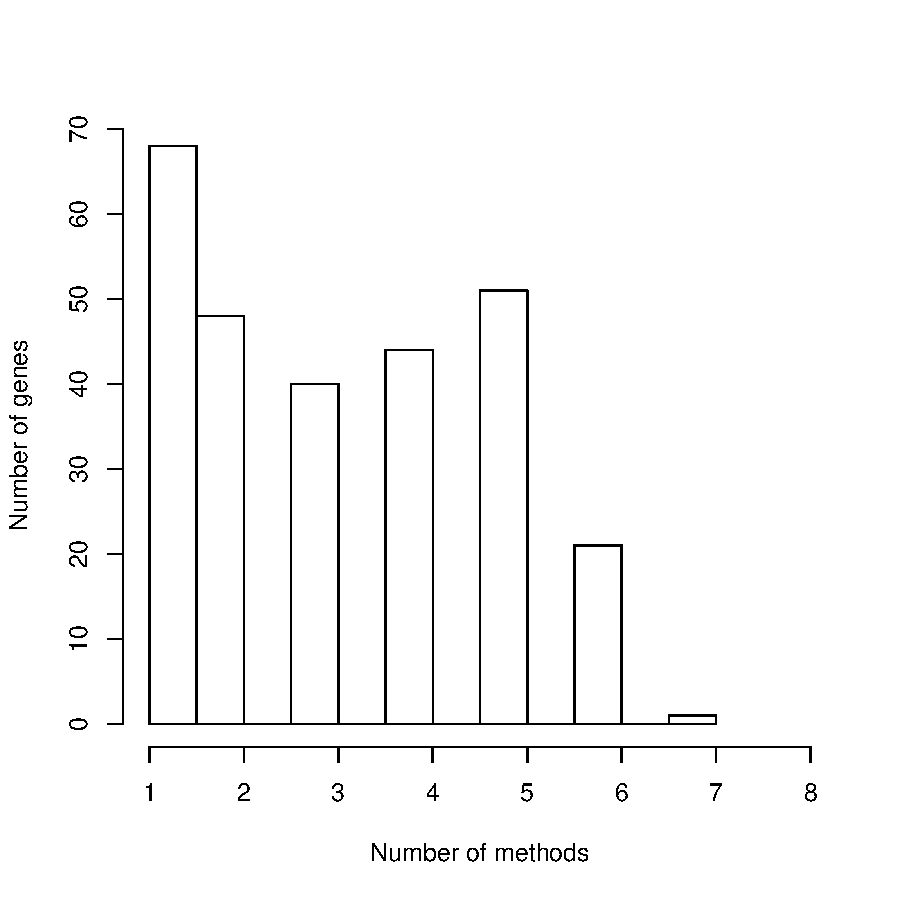
\includegraphics{MAMA_full-071}
\end{center}
{\ttfamily n.met} is a numeric vector of number of methods that identified the gene as differentially expressed. \par 
Next, we can look for example how many genes have been found as differentially expressed in at least 6 methods.
\begin{Schunk}
\begin{Sinput}
> dim(MAT[n.met>5,])
\end{Sinput}
\begin{Soutput}
[1] 22  7
\end{Soutput}
\end{Schunk}
On the other hand, we can find out how many genes have been found by a method.
\begin{center}
\begin{Schunk}
\begin{Sinput}
> n.gen<-apply(MAT,2,sum)
> barplot(n.gen, cex.names=0.8, las=2)
\end{Sinput}
\end{Schunk}
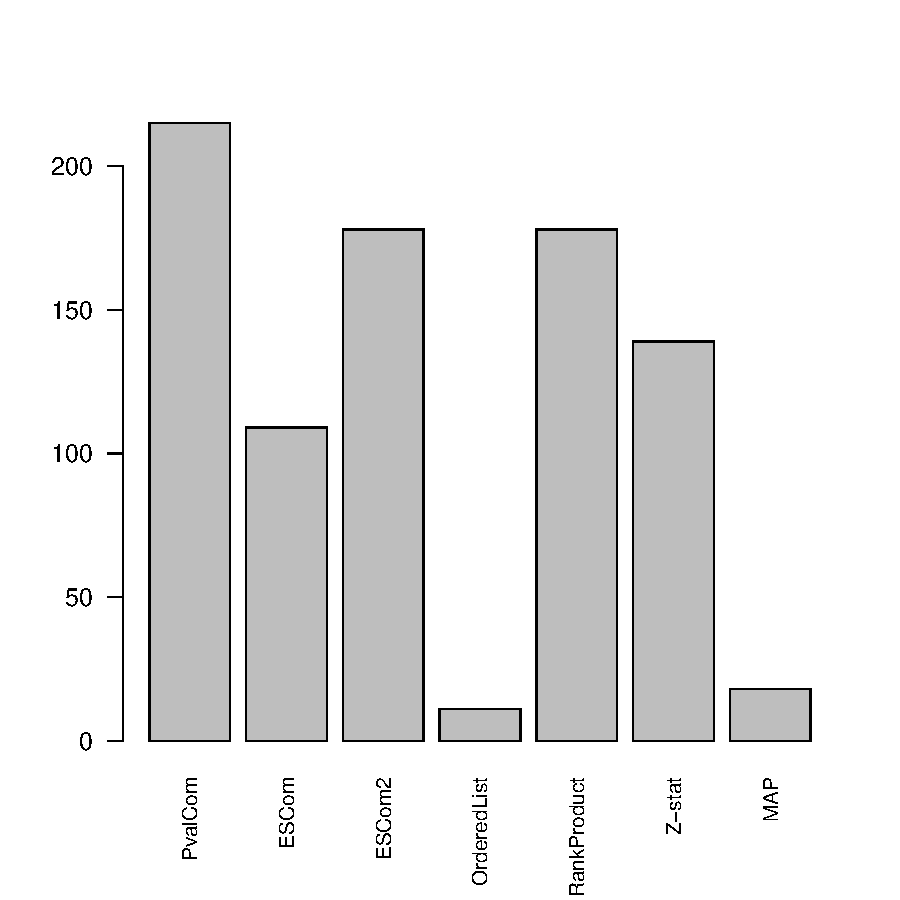
\includegraphics{MAMA_full-073}
\end{center}
Function {\ttfamily contig.tab} provides a number of genes common in two gene lists. It can be applied to {\ttfamily lists}, too.
\begin{Schunk}
\begin{Sinput}
> TAB<-conting.tab(lists)
> TAB[1:5,1:5]
\end{Sinput}
\begin{Soutput}
            PvalCom ESCom ESCom2 OrderedList RankProduct
PvalCom          NA   109    178          11         143
ESCom           109    NA    109          11          97
ESCom2          178   109     NA          11         134
OrderedList      11    11     11          NA          11
RankProduct     143    97    134          11          NA
\end{Soutput}
\end{Schunk}
%Integration Driven Discovery (IDD) and Integration Driven Revision (IDR) became popular for methods which combine p-values or effect sizes. IDD is a gene that has been found significant in meta-analysis but not in any of one data set analyses. A gene that is significant only in one data set analysis and not in meta-analysis is called IDR. A high number of IDD suggests that the method is capable to catch small but constant changes in gene expression, whereas high number of IDR is being explained as capability to suppress great expression changes observed in only one data set.\par % Function {\ttfamily makeIDDIDRtable()} provides IDD/IDR characteristic of all 

\section*{Expression of one gene}
In this section we are going to focus on one gene and to look at its expression change from different points of view. The different points of view are represented by different approaches used in the methods.\par
First we will join all the available results to one list and then select only rows for one gene.\par

\begin{Schunk}
\begin{Sinput}
> results<-join.results(pvalt, ESt, theScores, ScoresFDR$two.sided, SOGL.res,
+  RankRes, z.stat, probs, MC, RQ, type=c(1,1,5,5,2,3,5,4,5,5), 
+  genenames=rownames(GEDM(ColonData)[[1]]))
> #or 
> results2<-join.results(pval, es, es2, SOGL.res, rp, z.stat, map, metra)
> gene<-metagene("203008_x_at",results2)
> names(gene)<-c("pval","es.metaMA", "es.GeneMeta", "SOGL", "RP", "z.stat",
+  "MAP", "METRADISC")
> gene
\end{Sinput}
\begin{Soutput}
$pval
       study1        study2        study3 AllIndStudies 
     1.000000      1.000000      1.000000      1.000000 
         Meta TestStatistic 
     1.000000      8.732214 
attr(,"class")
[1] "metaMA"      "metaMA.gene"

$es.metaMA
       study1        study2        study3 AllIndStudies 
     1.000000      1.000000      1.000000      1.000000 
         Meta TestStatistic 
     1.000000     -8.492688 
attr(,"class")
[1] "metaMA"      "metaMA.gene"

$es.GeneMeta
     zSco_Ex_1      zSco_Ex_2      zSco_Ex_3           zSco 
 -6.4432924942  -3.7652548865  -4.6965956199  -8.8027593869 
        MUvals          MUsds          Qvals             df 
 -1.7730928661   0.2014246656   0.2626001205   2.0000000000 
      Qpvalues          Chisq    Effect_Ex_1    Effect_Ex_2 
  0.8769545957   0.0000000000  -1.7184785951  -2.0248658800 
   Effect_Ex_3 EffectVar_Ex_1 EffectVar_Ex_2 EffectVar_Ex_3 
 -1.7586784853   0.0711332351   0.2892036455   0.1402189026 
     zSco_Ex_1       FDR_Ex_1      zSco_Ex_2       FDR_Ex_2 
 -6.4432924942   0.0000000000  -3.7652548865   0.0325000000 
     zSco_Ex_3       FDR_Ex_3           zSco            FDR 
 -4.6965956199   0.0007142857  -8.8027593869   0.0000000000 
        MUvals          MUsds          Qvals             df 
 -1.7730928661   0.2014246656   0.2626001205   2.0000000000 
      Qpvalues          Chisq 
  0.8769545957   0.0000000000 
attr(,"class")
[1] "ES.GeneMeta"      "ES.GeneMeta.gene"

$SOGL
NULL
<0 rows> (or 0-length row.names)

$RP
        gene.index            RP/Rsum FC:(class1/class2) 
          415.0000            78.6607             0.5803 
               pfp            P.value 
            0.0000             0.0000 
attr(,"class")
[1] "RankProduct"      "RankProduct.gene"

$z.stat
              Zscore       Pvalue
203008_x_at 4.708621 2.493978e-06

$MAP
 110  101  011  111 
TRUE TRUE TRUE TRUE 
attr(,"class")
[1] "MAP.Matches"      "MAP.Matches.gene"

$METRADISC
 r.star  q.star  R.high   R.low  Q.high   Q.low 
497.000  38.000   0.000   1.000   0.998   0.002 
attr(,"class")
[1] "METRADISC"      "METRADISC.gene"

attr(,"class")
[1] "metagene"
\end{Soutput}
\end{Schunk}
This output provides much of the information available on the gene through all the described methods. It is a rather complicated structure, so we will try to represent it graphically in comprehensible form.
\begin{center}
\begin{Schunk}
\begin{Sinput}
> plotgene(gene, type=c(0,0,1,4,5,6,7,10), datalabels=c("denmark", "australia",
+  "japan", "combined"))
\end{Sinput}
\end{Schunk}
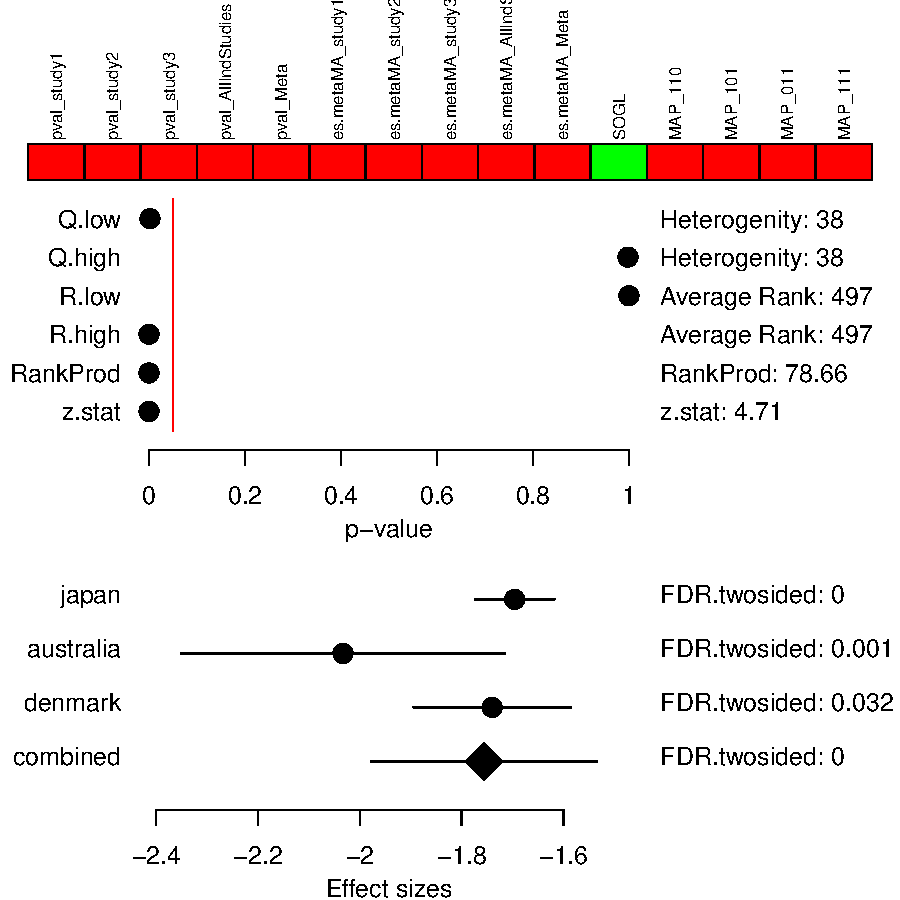
\includegraphics{MAMA_full-076}
\end{center}
The picture above shows in top part occurrence of gene in lists of selected genes in some methods.  The dark box means that the gene is present in the list. Values from objects: {\ttfamily pvalt}, {\ttfamily ESt}, {\ttfamily x.z} and {\ttfamily probs} are used in here. \par
The middle part is dedicated to p-values available in meta-analysis. Specific values of the statistics can be found on the right side of the chart. The vertical dashed line denotes the signifficance threshold $5\%$. P-values from {\ttfamily MC}, {\ttfamily RankRes} and {\ttfamily z.stat} are drawn in here.\par
Combination of effect size is plotted in the bottom graph. The point marks the effect size. Horizontal lines denote the variance of effect size. Statistical significance of the difference in gene expression (FDR adjusted) can be found on the right side of the chart. This graph uses values from {\ttfamily theScores} and {\ttfamily ScoresFDR}.

\begin{thebibliography}{99}
\bibitem{ausaden}Jorissen, R. N., Lipton, L., Gibbs, P., Chapman, M. et al. 2008, \emph{DNA copy-number alterations underlie gene expression differences between microsatellite stable and unstable colorectal cancers}, Clinical Cancer Research, Vol. 14, pp. 8061-8069
\bibitem{japan}Watanabe, T., Kobunai, T., Toda, E., Yamamoto, Y. et al. 2006, \emph{Distal colorectal cancers with microsatellite instability (MSI) display distinct gene expression profiles that are different from proximal MSI cancers} Cancer Research, Vol.66, no. 20, pp. 9804-9808
\bibitem{Biobase}Falcon, S., Morgan, M. and Gentleman, R. 2007, \emph{An introduction to Biocinductor's ExpressionSet class}, available at: http://www.bioconductor.org/packages/2.2/bioc/vignettes/Biobase/inst /doc/ExpressionSetIntroduction.pdf
\bibitem{Marot}Marot, G., Foulley, J.L., Mayer, C.D.,Jaffrezic, F. 2009, \emph{Moderated effect size and P-value combinations for microarray meta-analyses}, Bioinformatrics, Vol. 25 no. 20 2009, pp. 2692-2699
\bibitem{Rhodes}Rhodes, D.R., Barrette, T.R., Rubin, M. A., Ghosh, D. a Chinnaiyan, A. M. 2002, \emph{Meta-Analysis of Microarrays: Interstudy Validation of Gene Expression Profiles Reveals Pathway Dysregulation in Prostate Cancer}, CANCER RESEARCH 62, pp: 4427-4433
\bibitem{Fisher25}Fisher, R.A. 1925, \emph{Statistical methods for research}, Oliver and Boyd, Edinburgh
\bibitem{limma}Smyth, G. K. 2004, \emph{Linear models and empirical Bayes methods for assessing differential expression in microarray experiments}, Statistical Applications in Genetics and Molecular Biology 3, No. 1, Article 3
\bibitem{SMVar}Jaffrezic, F., Marot, G., Degrelle, S., Hue, I., Foulley, J.L. 2007, \emph{A structural mixed model for variances in differential gene expression studies}, Genetical Research, Vol. 89, pp. 19-25.
\bibitem{Choi2003}Choi, J.K., Yu, U., Kim, S. a Yoo, O.J. 2003, \emph{Combining multiple microarray studies and modeling interstudy variation}, Bioinformatics, Vol. 19, Suppl. 1 2003, pp. i84-i90
\bibitem{GeneMeta}Gentleman, R., Rauschhaupt, M., Huber, W., a Lusa L. 2008, \emph{Meta-analysis for Microarray Experiments}, available at: http://www.bioconductor.org/packages/2.3/bioc/vignettes/GeneMeta /inst/doc/GeneMeta.pdf 
\bibitem{Hedges}Hedged, V. L. a Olkin, I. 1985, \emph{Statistical Methods for Metaanalysis}, Academic Press, Orlando
\bibitem{Cochran}Cochran, B.G. 1954, \emph{The combination of estimates from different experiments}, Biometrics, Vol. 10, pp. 101-129
\bibitem{DerSimonian}DerSimonian, R., a Laird, N. M. 1986, \emph{Meta-analysis in clinical trials}, Controlled Clinical Trials, Vol. 7, pp. 177-188
\bibitem{SOGL}Scheid, S., Lottaz, C., Yang, X. a Spang, R. 2006, \emph{Similarities of Ordered Gene Lists User's Guide to the Bioconductor Package OrderedList 1.11.3}, availale at: http://www.bioconductor.org/packages/2.5/bioc/vignettes/
OrderedList/inst/doc/tr\_2006\_01.pdf
\bibitem{Hong}Hong, F., Breitling, R., McEntee,C. W., Wittner, B. S., Nemhauser, J. L. a Chory, J. 2006, \emph{RankProd: a bioconductor package for detecting differentially expressed genes in meta-analysis}, Bioinformatics, Vol. 22, no. 22 2006, pp. 2825-2827
\bibitem{Wang}Wang, J., Coombes, K. R., Highsmith, W. E., Keating, M. J. a  Abruzzo, L. V. 2004, \emph{Differences in gene expression between B-cell chronic lymphocytic leukemia and normal B cells: a meta-analysis of three microarray studies}, Bioinformatics, Vol. 20, no. 17 2004, pp. 3166-3178
\bibitem{metaArray} Ghosh, D. a Choi, H. 2009, \emph{metaArray package for meta-analysis of microarray data}, available at: http://bioconductor.org/packages/2.5/bioc/vignettes/metaArray/inst/ doc/metaArray.pdf
\bibitem{Geman}Geman, D., d'Avignon, Ch., Naiman, D. Q. a Winslow, R.L. 2004, \emph{Classifying Gene Expression Profiles from Pairwise mRNA Comparisons}, Statistical Applications in Genetics and Molecular Biology 2004, Vol. 3, Issue 1, Article 19
\bibitem{Tan} A.C. Tan, D.Q. Naiman, L. Xu, R.L. Winslow, D. Geman, \emph{Simple decision rules for classifying human cancers from gene expression profiles}, Bioinformatics, 21: 3896-3904, 2005.
\bibitem{Smid}Smid, M., Dorssers, L. C. J. a Jenster, G. 2003, \emph{Venn Mapping: clustering of heterologous microarray data based on the number of co-occurring differentially expressed genes}, Bioinformatics, Vol. 19, no. 16 2003, pp. 2065-2071
\bibitem{Yang2005}Yang, X., Bentink, S. a Spang, R. 2005, \emph{Detecting Common Gene Expression Patterns in Multiple Cancer Outcome Entities}, Biomedical Microdevices, Vol.7:3, pp. 247-251
\bibitem{velkyRhodes}Rhodes, D. R., Yu, J., Shanker, K., Deshpande, N., Varambally, R., Ghosh, D., Barrette, T., Pandey, A. a Chinnaiyan, A. M. 2004, \emph{Large-scale meta-analysis of cancer microarray data identifies common transcriptional profiles of neoplastic transformation and progression}, PNAS, Vol. 101, no. 25, pp. 9309-9314
\bibitem{Zintzaraz}Zintzaraz, E a Ioannidis, J.P.A. 2008, \emph{Meta-analysis for ranked discovery datasets: Theoretical framework and empirical demonstration for microarrays}, Computational Biology and Chemistry 32, pp. 39-47
%\bibitem{Heatplus}
%\bibitem{gplots}
\end{thebibliography}
\end{document}

